% Options for packages loaded elsewhere
% Options for packages loaded elsewhere
\PassOptionsToPackage{unicode}{hyperref}
\PassOptionsToPackage{hyphens}{url}
\PassOptionsToPackage{dvipsnames,svgnames,x11names}{xcolor}
%
\documentclass[
  a4paper,
  DIV=11,
  numbers=noendperiod,
  onecolumn,
  oneside,
  a4paper]{scrartcl}
\usepackage{xcolor}
\usepackage[lmargin=1in,rmargin=1in,tmargin=1in,bmargin=1in]{geometry}
\usepackage{amsmath,amssymb}
\setcounter{secnumdepth}{5}
\usepackage{iftex}
\ifPDFTeX
  \usepackage[T1]{fontenc}
  \usepackage[utf8]{inputenc}
  \usepackage{textcomp} % provide euro and other symbols
\else % if luatex or xetex
  \usepackage{unicode-math} % this also loads fontspec
  \defaultfontfeatures{Scale=MatchLowercase}
  \defaultfontfeatures[\rmfamily]{Ligatures=TeX,Scale=1}
\fi
\usepackage{lmodern}
\ifPDFTeX\else
  % xetex/luatex font selection
\fi
% Use upquote if available, for straight quotes in verbatim environments
\IfFileExists{upquote.sty}{\usepackage{upquote}}{}
\IfFileExists{microtype.sty}{% use microtype if available
  \usepackage[]{microtype}
  \UseMicrotypeSet[protrusion]{basicmath} % disable protrusion for tt fonts
}{}
\makeatletter
\@ifundefined{KOMAClassName}{% if non-KOMA class
  \IfFileExists{parskip.sty}{%
    \usepackage{parskip}
  }{% else
    \setlength{\parindent}{0pt}
    \setlength{\parskip}{6pt plus 2pt minus 1pt}}
}{% if KOMA class
  \KOMAoptions{parskip=half}}
\makeatother
% Make \paragraph and \subparagraph free-standing
\makeatletter
\ifx\paragraph\undefined\else
  \let\oldparagraph\paragraph
  \renewcommand{\paragraph}{
    \@ifstar
      \xxxParagraphStar
      \xxxParagraphNoStar
  }
  \newcommand{\xxxParagraphStar}[1]{\oldparagraph*{#1}\mbox{}}
  \newcommand{\xxxParagraphNoStar}[1]{\oldparagraph{#1}\mbox{}}
\fi
\ifx\subparagraph\undefined\else
  \let\oldsubparagraph\subparagraph
  \renewcommand{\subparagraph}{
    \@ifstar
      \xxxSubParagraphStar
      \xxxSubParagraphNoStar
  }
  \newcommand{\xxxSubParagraphStar}[1]{\oldsubparagraph*{#1}\mbox{}}
  \newcommand{\xxxSubParagraphNoStar}[1]{\oldsubparagraph{#1}\mbox{}}
\fi
\makeatother


\usepackage{longtable,booktabs,array}
\usepackage{calc} % for calculating minipage widths
% Correct order of tables after \paragraph or \subparagraph
\usepackage{etoolbox}
\makeatletter
\patchcmd\longtable{\par}{\if@noskipsec\mbox{}\fi\par}{}{}
\makeatother
% Allow footnotes in longtable head/foot
\IfFileExists{footnotehyper.sty}{\usepackage{footnotehyper}}{\usepackage{footnote}}
\makesavenoteenv{longtable}
\usepackage{graphicx}
\makeatletter
\newsavebox\pandoc@box
\newcommand*\pandocbounded[1]{% scales image to fit in text height/width
  \sbox\pandoc@box{#1}%
  \Gscale@div\@tempa{\textheight}{\dimexpr\ht\pandoc@box+\dp\pandoc@box\relax}%
  \Gscale@div\@tempb{\linewidth}{\wd\pandoc@box}%
  \ifdim\@tempb\p@<\@tempa\p@\let\@tempa\@tempb\fi% select the smaller of both
  \ifdim\@tempa\p@<\p@\scalebox{\@tempa}{\usebox\pandoc@box}%
  \else\usebox{\pandoc@box}%
  \fi%
}
% Set default figure placement to htbp
\def\fps@figure{htbp}
\makeatother





\setlength{\emergencystretch}{3em} % prevent overfull lines

\providecommand{\tightlist}{%
  \setlength{\itemsep}{0pt}\setlength{\parskip}{0pt}}



 


\usepackage[noblocks]{authblk}
\renewcommand*{\Authsep}{, }
\renewcommand*{\Authand}{, }
\renewcommand*{\Authands}{, }
\renewcommand\Affilfont{\small}
\KOMAoption{captions}{tableheading,figureheading}
\makeatletter
\@ifpackageloaded{caption}{}{\usepackage{caption}}
\AtBeginDocument{%
\ifdefined\contentsname
  \renewcommand*\contentsname{Table of contents}
\else
  \newcommand\contentsname{Table of contents}
\fi
\ifdefined\listfigurename
  \renewcommand*\listfigurename{List of Figures}
\else
  \newcommand\listfigurename{List of Figures}
\fi
\ifdefined\listtablename
  \renewcommand*\listtablename{List of Tables}
\else
  \newcommand\listtablename{List of Tables}
\fi
\ifdefined\figurename
  \renewcommand*\figurename{Figure}
\else
  \newcommand\figurename{Figure}
\fi
\ifdefined\tablename
  \renewcommand*\tablename{Table}
\else
  \newcommand\tablename{Table}
\fi
}
\@ifpackageloaded{float}{}{\usepackage{float}}
\floatstyle{ruled}
\@ifundefined{c@chapter}{\newfloat{codelisting}{h}{lop}}{\newfloat{codelisting}{h}{lop}[chapter]}
\floatname{codelisting}{Listing}
\newcommand*\listoflistings{\listof{codelisting}{List of Listings}}
\makeatother
\makeatletter
\makeatother
\makeatletter
\@ifpackageloaded{caption}{}{\usepackage{caption}}
\@ifpackageloaded{subcaption}{}{\usepackage{subcaption}}
\makeatother
\usepackage{bookmark}
\IfFileExists{xurl.sty}{\usepackage{xurl}}{} % add URL line breaks if available
\urlstyle{same}
\hypersetup{
  pdftitle={Bachelor Thesis},
  pdfauthor={© Benjamin Gross},
  colorlinks=true,
  linkcolor={blue},
  filecolor={magenta},
  citecolor={magenta},
  urlcolor={blue},
  pdfcreator={LaTeX via pandoc}}


\title{Bachelor Thesis}
\usepackage{etoolbox}
\makeatletter
\providecommand{\subtitle}[1]{% add subtitle to \maketitle
  \apptocmd{\@title}{\par {\large #1 \par}}{}{}
}
\makeatother
\subtitle{Gesundheit und Management}
\author{© Benjamin Gross}
\date{23.04.2026 07:33}
\begin{document}
\maketitle
\begin{abstract}
Die vorliegende Arbeit beschäftigt sich mit dem Serious Game Prototypen
BenBox.org, ein Spiel für Kinder der Zielgruppe 6 bis 13 Jahre, in der
Gesundheitsförderung im deutschen eHealth-Markt. Der verwendete
Prototyp, in Form eines Exergames, schult über motorische Interventionen
das Bewegungsverhalten der Nutzer.
\end{abstract}

\renewcommand*\contentsname{Table of contents}
{
\hypersetup{linkcolor=}
\setcounter{tocdepth}{5}
\tableofcontents
}

!{[}Ein Bild, das Objekt enthält.

Mit hoher Zuverlässigkeit generierte
Beschreibung{]}(resources/images/image1.jpeg)

Fachbereich Gesundheit \& Soziales

Gesundheit und Management für Gesundheitsberufe (B. Sc.)

Standort: Köln

\textbf{BenBox.org }

\textbf{Untersuchung eines 'Serious Game` in Bezug auf seinen Nutzen in
der Gesundheitsförderung}

Bachelor-Arbeit zur Erlangung des Akademischen Grades

„Bachelor of Science`` (B. Sc.)

Benjamin Groß

400147257

Erstgutachter: Herr Dr. Robert Zickermann

Zweitgutachter: Herr Prof. Dr. Hans-Hermann Dirksen

Semester: SS 2019

11.06.2019

Inhaltsverzeichnis

Zusammenfassung 1

Abkürzungsverzeichnis 2

Abbildungsverzeichnis 3

1 Einleitung 4

2 Aktueller Forschungsstand 7

3 Methode 10

\begin{verbatim}
3\.1    Erhebung der Daten                              12

3\.2    Auswertung der Daten                            14
\end{verbatim}

4 Nutzen Digitaler Medien 15

4.1 Serious Games in der Edukation (eLearning) 19

4.2 Serious Games in der Gesundheitsförderung (eHealth) 23

\begin{verbatim}
4\.3    Ökonomische Betrachtungen eines Serious Games           27

    4\.3\.1 Vertriebswege                           29

    4\.3\.2 Finanzierungsstrategien                     31

    4\.3\.3 Vertriebs\-, Finanzierungs\- und Marketingmix           32

4\.4    Ökonomische Betrachtungen eines Corporate Games         34
\end{verbatim}

5 Ergebnisse 34

6 Diskussion 37

7 Fazit und Ausblick 41

Literaturverzeichnis 44

Anhang 51

Eidesstattliche Versicherung 58

\section{Zusammenfassung}\label{zusammenfassung}

Die vorliegende Arbeit beschäftigt sich mit dem Serious Game Prototypen
BenBox.org, ein Spiel für Kinder der Zielgruppe 6 bis 13 Jahre, in der
Gesundheitsförderung im deutschen eHealth-Markt. Der verwendete
Prototyp, in Form eines Exergames, schult über motorische Interventionen
das Bewegungsverhalten der Nutzer. In seiner erweiterten eLearning
Funktion vermittelt das Serious Game über den Spielerzählstrang
Kenntnisse in Religions- und Geschichtswissenschaft.

Das Augenmerk dieser empirischen Arbeit liegt auf der ökonomischen
Sinnhaftigkeit dieses eHealth-Angebotes. Im Rahmen einer durchgeführten
Umfrage, verknüpft mit dem Spiele-Test des BenBox.org Prototypen, wurden
Daten von Schülern einer dritten Klasse erhoben. Die Kinder im Alter von
acht und neun Jahren wurden in Paarungen an einem iPad Pro mit dem
Exergame konfrontiert und im Spielverlauf zu ihren Erfahrungen befragt.

Der Nutzen digitaler Medien, insbesondere die ökonomische Betrachtung
eines solchen eHealth-Produktes, wird anschließend von Seiten des
Vertriebsweges, der Finanzierbarkeit und des Marketings reflektiert.
Dazu werden die gesammelten Umfrageergebnisse mit dem aktuellen
wissenschaftlichen Diskurs verglichen, sowie die gängigen ökonomischen
Ansätze des Marktes betrachtet. Zu diesen Zwecken werden die für
digitale Produkte zurzeit verfügbaren Monetarisierungsstrategien,
Finanzierungsquellen, sowie Marketingstrategien sondiert, im
Diskussions-Teil auf das BenBox.org Spiel übertragen und daraus
abgeleitet ein Finanzplan erstellt. Im Schlussteil dieser Arbeit wird
die konkrete zukünftige Realisation der anvisierten technischen und
monetären Ziele des Projektes beschrieben.

\textbf{Schlüsselwörter:} Serious Game, Exergame, Prototyp, Spiele-Test,
Kinder, Gesundheitsförderung, eHealth, eLearning, Umfrage, Ökonomie,
Vertrieb, Finanzierung, Marketing, Monetarisierungsstrategien,
Finanzplan

\section{Abkürzungsverzeichnis}\label{abkuxfcrzungsverzeichnis}

eBooks elektronische / digitale Bücher

eHealth elektronische / digitale Gesundheitsprodukte

eLearning digitales Lernen

GKV Gesetzliche Krankenkassen

KI Künstliche Intelligenz

NPC Non-player character

PI Persönliche Intelligenz

PKV Private Krankenkasse

Prg Paarung

Tablet Tablet-Computer

TK Techniker Krankenkasse

UI User Interface

VR Virtual Reality

ZPP Zentrale Prüfstelle für Prävention

\section{Abbildungsverzeichnis}\label{abbildungsverzeichnis}

Abb. 1.1: Serious Games für Weiterbildungen S. 6

Abb. 4.1: Durchschnittlicher App-Preis S. 16

Abb. 4.2: Durchschnittliche Spiele-Preise S. 17

Abb. 4.2.1: Angeborene Lernlust S. 24

Abb. 4.3.1: Produktion von Gesundheitsprodukten S. 28

Abb. 4.3.2.1: Budgetplan ‚Bolt Riley Episode 1` S. 32

Abb. 5.1: Item 1 S. 35

Abb. 5.2: Item 2 S. 35

Abb. 5.3: Item 3 S. 36

Abb. 5.4: Item 4 S. 36

Abb. 5.5: Item 5 S. 36

Abb. 6.1: Tabelle -- Produktionskosten S. 39

Abb. 6.2: Tabelle -- Kapitalquellen S. 39

\section{1 Einleitung}\label{einleitung}

Digitalisierung und ihre Begleitthemen, wie Datenschutz, Big Data,
Verschlüsselung, Blockchain, Cloud-Dienste, Deep Learning, Internet of
Things (IoT), Augmented Reality und Virtual Reality (VR), Gamification,
Robotik, Assistenz-Systeme wie z.B. Siri und autonomes Fahren, sowie
Künstliche Intelligenz (KI) sind in aller Munde. Gerade das Thema der KI
und das Drohen wegfallender Jobs wird zum emotional aufgeladenen
Zukunftsszenario. Man geht davon aus, dass Berufe wie der des
Versicherungsmaklers, eine Tätigkeit, die sich ausschließlich mit
formalisierbaren Datensätzen beschäftigt, als erstes wegfallen und durch
eine spezialisierte schwache KI ersetzt werden. Die starke KI, welche
nicht nur für einen konkreten Anwendungsfall konstruiert ist und
Intelligenz nicht einfach simuliert, sondern dem Menschen ebenbürtig,
wenn nicht sogar überlegen ist, wird in absehbarer Zeit der
Science-Fiction Literatur vorbehalten sein (Informatik und Gesellschaft,
2009). Nach Russel und Norvig (2009) sind die Kennzeichen für eine
solche starke KI logisches Denken, Treffen von Entscheidungen bei
Unsicherheit, Planen, Lernen, Kommunikation in natürlicher Sprache,
sowie die Kombination all dieser Fähigkeiten zur Erreichung eines
gemeinsamen Ziels. Persönliche Intelligenz (PI) ist nach von Reventlow
und Thesen (2019) ein Assistenzsystems, dass dem Nutzer Vorschläge
unterbreitet, ihn unterstützt und das Leben vereinfacht.

Land (2018) zufolge bewegt sich die Menschheit auf dem Weg zur
Verwirklichung dieser Technologie durch fünf aufeinanderfolgende
industrielle Phasen: Mechanisierung, Elektrifizierung, Automatisierung
und Globalisierung, Digitalisierung und Vernetzung mit IoT, sowie
schlussendlich die Entwicklung von cyberphysischen Systemen.
Cyberphysische Systeme nutzen die Kooperation zwischen Mensch, Maschine
und Künstlicher Intelligenz, um effektiv und effizient Prozesse der
Herstellung oder Dienstleistung zu optimieren. Daher ist also nicht
verwunderlich, dass sich auch die Gesundheitsanbieter, die bekanntlich
mit knappen Ressourcen aus den Sozialtöpfen arbeiten müssen, ebenso mit
Digitalisierung und der Verwendung von KI auseinandersetzen. Auch werden
in diesem Bestreben immer mehr Mixed-Realtity-Umgebungen geschaffen.
Dabei handelt es sich um die Verknüpfung von Elementen der virtuellen
mit denen der realen Welt. Das kann z.B. ein realer Gegenstand sein, der
zusätzlich in der virtuellen Welt abgebildet wird und sich dort ganz
ähnlich verhält wie unter normalen physikalischen Bedingungen. Im
medizinischen Bereich kann so z.B. das Erproben von Operationsverfahren
ermöglicht werden. Diese Bestrebungen finden ihre Zusammenfassung in dem
Begriff elektronische bzw. digitale Gesundheitsprodukte (eHealth).

Die neueste Version der Apple Watch kann seit März 2019 auch in
Deutschland eine EKG-Messung durchführen und erfassen, ob ein normaler
Sinusrhythmus vorliegt. Die von Stanford Medicine veröffentlichte Apple
Heart Study belegt die Korrektheit der Daten der Apple Watch 4, die
mittels Fingersensor EKG-Messungen durchführt. Hiermit durchdringt die
Gesundheitsfürsorge letztendlich den Consumer Electronics Markt, also
den hart umkämpften Absatzmarkt für elektronische Geräte, der bisher von
großen Tech-Riesen wie Google, Microsoft, Samsung, und Apple dominiert
wird. Die Digitalisierung der Medizin, mit Diensten wie der
‚Doc-on-Demand`, einer Plattform, auf der ein Leistungserbringer zeit-
und ortsunabhängig zum medizinischen Rat zur Verfügung steht, ist in den
USA mit deutlichen Steigerungsraten versehen. Im Jahr 2015 verwendeten
schon über 85\% der niedergelassenen Ärzte und 90\% der Kliniken
digitale Patientenakten (Schmitt-Sausen, 2018). Die Zielgruppe dieser
Technologien ist altersübergreifend. Auch für Kinder werden eine
Vielzahl von elektronischen und digitalen Angeboten geschaffen. Einige
davon versprechen digitale Lernförderung, welche unter dem Begriff
eLearning zusammengefasst werden. Ebenso loben viele dieser Angebote
aus, dass ihre Verwendung zur Gesundheitsprophylaxe dient. Diese
Produkte für die junge Zielgruppe Kinder und Jugendliche, sind oftmals
für mobile Endgeräte entwickelt und bieten nicht selten eine eigene
Spielgeschichte mit Protagonisten. Diese Spielwelten sind häufig im
Comic-Stil verfasst. Allerdings muss berücksichtigt werden, dass Kinder
von den neuen Medien meist vor vollendete technische und erzählerische
Tatsachen gestellt werden. Moderne Unterhaltungsmedien verlangen den
jungen Menschen nicht selten sehr viel ab. Gerade bei spielerischen
Inhalten findet meist in kurzer Zeit eine Menge an Handlung, die
sogenannte ‚Action` statt. Diese kann vom Kind teilweise nur sehr
schwer, wenn überhaupt, emotional verarbeitet werden (Daun, 2012). So
steht die Frage im Raum, ob digitale Medien nutzbringend für die
Gesundheitsvorsorge von Kindern eingesetzt werden können oder diese im
schlechtesten Fall mit weiteren Stressoren belasten. Martin-Niedecken
und Mekler (2018) konstatieren die weitläufige Verbreitung dieser
Ansätze, geben jedoch zu bedenken, dass diese Technologien Schwächen
aufweisen im Vergleich zu klassischen Angeboten. Schlüsselwörter im
Bereich der motorischen Lernspiele seien ihnen zufolge ‚Embodiment`
‚Bodily Interplay` und ‚Presence`. Diese Aspekte des menschlichen
Lernens und der Entwicklung sind nicht zuletzt in den
somatopädagogischen Disziplinen wie Feldenkrais, Eutonie Gerda Alexander
und Qi-Gong relevant (Steinmüller, Schaefer \& Fortwängler, 2009).

Wirtschaftlicher Erfolg ist gerade auch von Literatur und
Unterhaltungsmedien der Kinder- und Jugendzielgruppe zu erwarten.
Prominentes Beispiel ist die Fantasy-Kinderbuch-Reihe ‚Harry Potter`.
Bücher, Filme, analoge und digitale Spiele über den Zauberlehrling und
seine Freunde, aus der Feder der britischen Autorin Joanne K. Rowling,
generierten Milliardenumsätze. Untersuchungen zeigen, dass Kinder im
Durchschnittsalter von neun Jahren ihr erstes ‚Harry Potter` Buch lasen.
Über 50 \% der Fünf- bis Siebzehnjährigen haben die Romane gelesen. Die
Altersgruppen neun bis elf und 12 bis 14 Jahre sind die eifrigsten Leser
und somit am stärksten für den Erfolg der Serie verantwortlich (Egger,
2009). Hinsichtlich der Digitalisierung, ist zu beobachten, dass alle
großen Anbieter neben den klassischen Hörspielen insbesondere Spiele für
Handy, Tablet-Computer (Tablet) und PC-System herausbringen, die dann
zum Download verfügbar sind. Neben konventionellen Spielen werden
digitale Medien auch zu Lernzwecken eingesetzt. Oftmals sind die
Lerninhalte mit Gamification-Elementen angereichert, sodass eine
durchgeführte Handlung in einer Belohnung in Form von Punkten und
dergleichen mündet. Ist das digitale Medium jedoch grundsätzlich als
Spiel konzipiert, vermittelt allerdings Wissen oder schult sinnvolles
Verhalten, spricht man von einem Serious Game. Bei Spielen die
überwiegend auf die körperliche Ertüchtigung abzielen auch von einem
Exergame. Zuerst benutzte Clark Abt 1970 den Begriff Serious Game und
beschrieb ihn mit „Nicht beabsichtigt um primär zum Vergnügen gespielt
zu werden`` (Schmitt, Christopher, Tumanov, Weiss \& Möckel, 2018).
Kommen diese Sorte Spiele im Unternehmensumfeld zu Schulungszwecken zum
Einsatz, ist von einem Corporate Game die Rede. Letzterer Begriff deutet
darauf hin, dass Serious Games auch in Unternehmen eingesetzt werden, um
Mitarbeiter mittels des gemeinsamen spielerischen Lernens, z.B. im
Umgang mit Industrie-Applikationen oder in der Gesundheitsprophylaxe zu
schulen. Wie in Abb. 1.1 zu ersehen, ist sich ein Großteil der
Personalverantwortlichen der Existenz von Serious Games im Kontext des
Lernens im Unternehmen bewusst, mehr als die Hälfte setzt diese Form der
Edukation bereits ein.

Abb. 1.1: Serious Games für Weiterbildungen

\pandocbounded{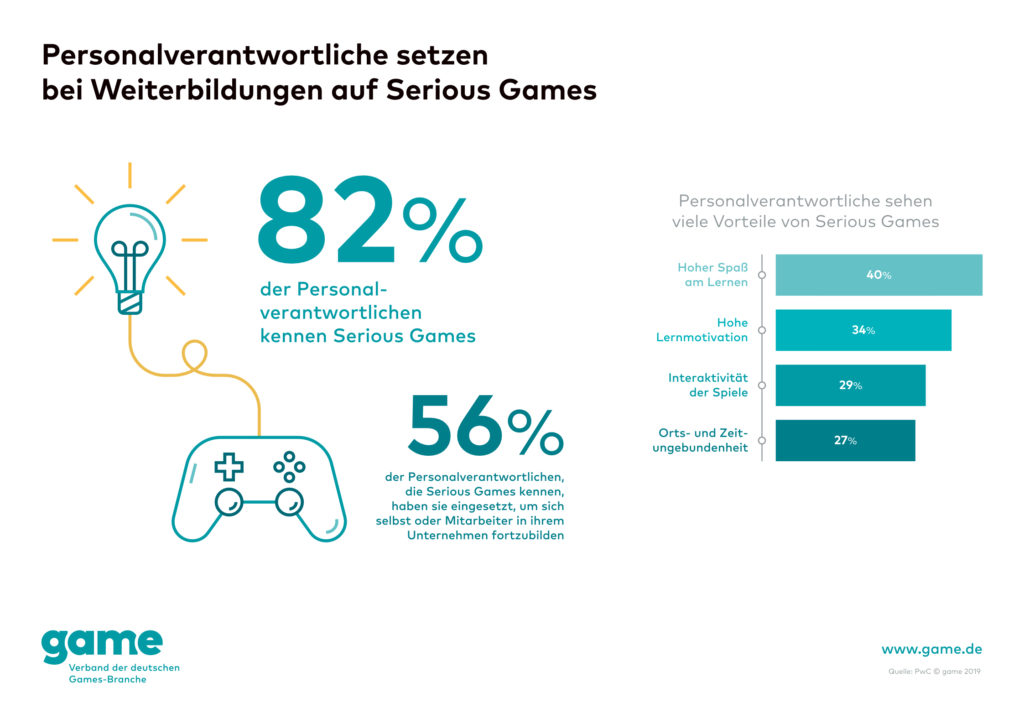
\includegraphics[keepaspectratio]{resources/images/image2.jpeg}}

Quelle: game -- Verband der deutschen Games-Branche e.V., 2018

Bedarf besteht definitiv nicht nur in der Schulung in neuen
Arbeitsmethoden, sondern auch in der Vorbeugung von Erkrankungen des
Muskelskelettsystems. Laut der AOK sind 2015 ein Drittel der Patienten,
die physiotherapeutische Behandlungen in Anspruch genommen haben, von
Rückenschmerzen betroffen gewesen. 2011 gaben 65 \% der Kinderärzte in
einer Umfrage von Statista an, dass Kinder und Jugendliche in den
letzten zehn Jahren mehr Rückenschmerzen beklagten. 88 \% der Ärzte
bemängelten darüber hinaus die sich verschlechternden koordinativen
Fähigkeiten und sprachen von manifesten motorischen Defiziten. Im
Hinblick auf diese Zahlen ist es verwunderlich, dass Kinder häufig in
sportpädagogischen Gruppen und eher selten in therapeutischen
Interventionen anzutreffen sind.

Die Boston Consulting Group hat in einer Studie die Region Köln-Bonn als
Digital-Health-Cluster untersucht. Mit sechs Millionen Versicherten und
einem starken Netzwerk an Gesundheitsdienstleistern, 57 Krankenhäusern,
\textasciitilde17.000 Betten und \textasciitilde686.000
Patienteneinweisungen innerhalb von 35 km Radius im Jahr 2016 ist eine
nennenswerte Gesundheits-Infrastruktur vorhanden. In Köln sind mehr als
650 Start-Ups und ca. 9.000 Beschäftigten sowie ca. eine Milliarde Euro
Umsatz angesiedelt, unter ihnen auch erfolgreiche eHealth-Anbieter. Dies
lässt im Hinblick auf die Vermarktung eines eHealth-Produktes auf ein
probates Netzwerk hoffen. Die TU Darmstadt gilt in Deutschland als das
Flaggschiff der Digitalforschung. Das Studienfach Multimedia
Kommunikation, angesiedelt im Fachbereich Elektrotechnik und
Informationstechnik, verfolgt die Vision der nahtlosen Kommunikation und
erforscht auch vielfältige Ansätze im Bereich eHealth. So kommen zu den
prognostizierten Wachstumsraten der Gesundheitsbranche im Digitalsektor
auch die entsprechenden Fachkräfte auf den Markt.

Unter Berücksichtigung dieser Erkenntnisse und aktueller
Forschungsergebnisse entsteht folgende Zielformulierung: Die vorliegende
Arbeit soll den aktuellen eHealth Markt, im Besonderen den
Gesundheits-Spielemarkt beleuchten, den Sachverhalt prüfen, ob das
digitale Medium ‚Serious Game` in der Gesundheitsförderung von Kindern
bisher eingesetzt wird, sowie ökonomisch erfolgversprechend vertrieben
werden kann. Hierzu muss grundsätzlich die Frage erläutert werden, was
die Gesundheit eines Kindes für einen monetären Wert hat, um eine
betriebswirtschaftliche Perspektive zu schaffen.

\section{2 Aktueller Forschungsstand}\label{aktueller-forschungsstand}

Strotbaum und Reiß (2017) fordern eine wissenschaftliche
Auseinandersetzung mit digitalen Medien, wie z.B. Gesundheits-Apps,
derer eine schier endlose Zahl in App-Stores zum Download angeboten
werden. So soll der Nutzer leichter eine Qualitätseinschätzung tätigen
können, sowie in seiner Mediennutzungskompetenz gestärkt werden. Gerade
Kinder weisen eine immer stärkere Neigung zur Handynutzung auf, wobei
sie hauptsächlich Videos konsumieren. Die Mediennutzungszeit steigt
weiterhin in allen Altersgruppen an, insbesondere die inhaltliche
Internetnutzung, sprich der Zugriff auf Medieninhalte. Insgesamt
schlagen pro Person zehn Stunden, samt Individualkommunikation zu Buche.
Diese hohe Zeitspanne entsteht allerdings durch die Parallelnutzung
verschiedener medialer Kanäle, wie z.B. die Handynutzung bei
gleichzeitigem Fernsehen (Adler, Ganzenberg, Martin, González \&
Schubert, 2017). Aus marketingorientierter Sicht wird die sonst schwer
zu erreichende Zielgruppe von Minderjährigen, mittels Apps und
kindgerechter Videos leichter erschließbar. Von den Zwölf- bis
Dreizehnjährigen verfügen 85 \% über ein eigenes Handy, dies macht die
Verbreitung von App-Angeboten potentiell lukrativ. Der finanzielle
Aufwand eines einfach konzipierten Lernprogramms für Apple und Android
Geräte ist dank moderner Entwicklungsumgebungen kalkulierbar geworden
und erfordert nach einer Studie aus 2015 des Fachdienstes iBusiness über
die Entwicklungskosten von Apps, nicht zwingend eine fünfstellige
Investition. Viele solcher Produkte sind anschließend werbefinanziert.
Als Beispiel sei die Webseite Toggo genannt. Toggo ist ein
Programmfenster für Kindersendungen des Privat Fernsehsenders Super RTL
und bietet kostenlose interaktive Browser Games an. Super RTL verwendet
dazu als Vorlage die eigenen Kinderserien und gestaltet sogenannte
Minigames mit minimalen Funktionsumfang und entsprechend niedrigen
Entwicklungskosten. Dazu schaltet der Anbieter an ihre Zielgruppe
angepasste Werbung. In diesem wachsenden digitalen Markt entsteht
zurzeit im Gesundheitsdienstleistungssektor eine Nische, also im
eHealth-Markt. Die benannten Serious Games sollen laut Krankenkassen
klassische Spielelemente mit evidenzbasierter Gesundheitsförderung
kombinieren, um die Motivation an Gesundheitsförderung zu steigern.
Start-Ups und am Markt etablierte Anbieter, die sich auf diese
Verquickung von Spiel und (Gesundheits-)Lernen spezialisieren, müssen
jedoch die medizinische Sinnhaftigkeit im Blick behalten und
gegebenenfalls belegen, um nicht einem rein betriebswirtschaftlichen
Streben zu unterliegen wie der zuvor genannte Absatzmarkt für
Unterhaltungsmedien (Strotbaum \& Reiß, 2017).

Mit der App ‚neolino`, welche auf der Webseite der Techniker
Krankenkasse (TK) beworben wird, können drei bis sieben Jährige, sofern
sie in logopädischer Behandlung und bei der TK versichert sind,
kostenlos zu Hause an der Verbesserung der Artikulation arbeiten
(Techniker Krankenkasse, 2019). Die TK ist mit über zehn Millionen
Versicherten, wovon 2,5 Millionen Familienversichert sind, die größte
Gesetzliche Krankenkasse (GKV) in Deutschland (Euro-Informationen,
2019). Nach Angaben der AOK sind im Jahre 2015 knapp ein Drittel ihrer
Patienten mit der Diagnose Rückenschmerz in physiotherapeutischer
Behandlung gewesen. In einer systematischen Übersichtsarbeit von 2019
von den Forschern Arnold, La Barrie, DaSilva, Patti, Goode und Clewley
wurde die Wirksamkeit von physiotherapeutischer Behandlung in den ersten
30 Tagen nach dem Auftreten des Schmerzes belegt. Die Kostenträger, also
die Krankenkassen, sowie im Unternehmen die Personalabteilung, sollten
solchen Angeboten dementsprechend offen gegenüberstehen, um
Dienstausfall ihrer Mitarbeiter vorzubeugen. So ist anzunehmen, dass die
Krankenkassen den Wert von Gesundheit monetär beziffern können, dies
differenziert für die Altersgruppen Kinder, Erwachsene und Senioren.
Nach Häckl (2010) sollte hierzu allerdings eine gesellschaftliche
Perspektive eingenommen werden, welche alle Kosten- und Nutzenpositionen
der Akteure berücksichtigt, um allgemeingültige Aussagen treffen zu
können.

Kursangebote zur Prävention wie Rückenschule sind ein klassisches
Angebot, um Rückenschmerzen vorzubeugen und bestehende Beschwerden zu
lindern. Wird solch ein Präventionsangebot durch die Zentrale Prüfstelle
für Prävention zertifiziert, können für Kinder und Erwachsene
Versicherungszuschüsse erwirkt werden. Serious Games, für die Zielgruppe
Kinder und Jugendliche, zu diesem Thema, die förderberechtigt sind, sind
bisher allerdings noch keine veröffentlicht. Daraus resultierend, ist in
diesem Marktsegment besagte Nische zu verzeichnen. Diese besteht
augenblicklich sowohl in der Angebotsverfügbarkeit als auch in der
betriebswirtschaftlichen Forschung über ebensolche Serious Games für
Kinder in der präventiven Gesundheitsförderung.

An dieser Stelle wird die Forschungsfrage wie folgt beschrieben werden:
„Wie kann ein Serious Game für Gesundheit für Kinder eingesetzt werden,
damit ökonomischer Erfolg generiert wird?{}``. Hierbei soll als
ökonomischer Erfolg gelten, wenn eine Gewinnmaximierung erzielt,
monetärer Erfolg für den Unternehmer und das Unternehmen umgesetzt,
nachhaltige und langfriste Planung in Hinblick auf die
Mitarbeiterbindung und Kompetenzsicherung im Unternehmen erreicht, sowie
die Diversifizierung der Produkte im Sinne eines Risikomanagements
durchgeführt wird. Die im Rahmen dieser Arbeit durchgeführte Umfrage
soll in Kapitel 5 Ergebnisse aus der Verwendung des BenBox.org
Prototypen liefern. Aus diesen Daten soll abgeleitet werden, ob ein
ökonomischer Nutzen, nach Strotbaum und Reiß (2017) als Effizienz der
unternehmerischen Bestrebungen definiert, für das Spiel zu erwarten ist.
Ebenso geklärt wird, welche Bestrebungen im Vertrieb, in der
Finanzierung und im Marketing unternommen werden müssen, um diese
Effizienz zu erreichen. Als Nebenfrage dient die ökonomische Betrachtung
von Serious Games für Arbeitnehmer im betrieblichen Umfeld, in dieser
Arbeit der übersichtlichkeitshalber mit der Bezeichnung ‚Corporate
Games` versehen.

\section{3 Methode}\label{methode}

Die vorliegende Arbeit ist empirischer Natur und soll Erfahrungen
bezüglich der Verwendung eines Spieles für Kinder im Bereich der
Gesundheitsförderung generieren. Im Vorfeld wurde das BenBox.org Serious
Game für Gesundheit als Prototyp für ein Apple iPad Pro entwickelt. Das
Spiel ist in Teilen in einer frühen Entwurfsphase und verwendet
teilweise semi-professionelle Darstellungen und Medien. Die
erforderlichen Informationen und Fachliteratur für den theoretischen
Teil dieser Arbeit wurden in Form von Büchern, elektronischen Büchern
(eBooks) und Journalen gewonnen. Die verwendeten eBooks sind teilweise
mit einer temporären Lizenz eingeschränkt, andere wiederum als
dauerhafte Kopie vorhanden. Die verschiedenen wissenschaftlichen Werke
wurden mittels Suche in Bibliotheksdatenbanken über entsprechende
Schlagwörter gefunden. Durch die Kombination unterschiedlicher, in
Beziehung zu einander stehender Schlagwörter, war es z.B. möglich,
Literatur über Healthcare-Angebote zu finden, die im Speziellen eine
Betrachtung von digitalen Gesundheits-Angeboten (eHealth) enthielt.
Einige der verwendeten Bücher und Journale befinden sich in der
persönlichen Sammlung des Autors. Zusätzlich wurde mit einer
Online-Suche im Internet recherchiert, um tagesaktuelle
Informationsquellen zu zitieren. Alle Online-Artikel mit Relevanz für
die vorliegende Arbeit sind als PDF gespeichert worden und liegen als
Hardcopy digital vor. Des Weiteren kamen statistische Daten von
Fremdanbietern zum Einsatz. Diese Daten waren insofern von Bedeutung, da
die veränderte Mediennutzung mittlerweile erfasst ist und dadurch eine
hohe Aussagekraft bezüglich des Einsatzes von digitalen Medien möglich
ist. Solche Datensätze werden z.B. vom Bundesamt für Statistik erhoben
und jährlich veröffentlicht.

Fragebogen als Begriff wird häufig verwendet, obwohl die Grundlagen
dieses Instrumentes nur selten systematisch berücksichtigt werden
(Kallus, 2016). Nach Hennings (2012) muss zur Überprüfung einer zeitlich
gesehen früher definierten Hypothese, ein komplexer Ablauf der
Untersuchung eingehalten werden. Erst dann kann von einer systematischen
Erhebung ausgegangen werden. Der vorliegende Fragebogen ist den
Empfehlungen der Literatur weitestgehend gefolgt, allerdings wurden, der
Kürze dieser Arbeit geschuldet, keine zuvor standardisierten
Fragestellungen verwendet. Um die sprachliche Verständlichkeit zu
gewährleisten, wurden nur positive Formulierungen eingesetzt und
gänzlich auf komplizierte Satzkonstruktionen verzichtet (Kevala, 2012).
So kann nach Porst (2014) die Syntax jeder Frage leicht verstanden
werden, sowie sämtliche Begriffe und Inhalte der Umfrage Items begriffen
und der Sinn vollständig erfasst werden. Insbesondere wurden die Fragen
in dieser Umfrage dem Sprachgebrauch von Kindern angepasst. Die Fragen-
und Antwortmöglichkeiten wurden keiner vorherigen Überprüfung und
Erprobung unterzogen. Im Rahmen dieser Arbeit wird daher von einer
Umfrage gesprochen, da den hohen wissenschaftlichen Ansprüchen eines
standardisierten Fragebogens nicht entsprochen wird.

Die Umfrage hat eine zweiteilige Gliederung. Über einen Einleitungsteil,
der über den Sinn der Studie informiert, musste die Umfrage nicht
verfügen, da im Vorfeld ein Informend Consent an die Eltern der
Schulkinder ausgeteilt wurde. Die Erziehungsberechtigten wurden
detailliert über den Ablauf der Studie informiert und über das Ziel
dieser Arbeit aufgeklärt. Alle Fragen aus der Umfrage waren
obligatorisch, d.h. die Fragen mussten von den Befragten beantwortet
werden. Auf diese Weise sollten ungültige Umfrageergebnisse
ausgeschlossen werden. Die Umfrage enthielt ausschließlich quantitative
Fragen. Im Gegensatz zu geführten Interviews, können quantitative Fragen
mit einem geringen zeitlichen und finanziellen Aufwand betrieben werden
(Hennings, 2012). Die Umfrage wurde als eine Stichprobenbeobachtung
durchgeführt, mit dem Ziel auf die Grundgesamtheit der entsprechenden
Altersgruppe schließen zu lassen. Solange diese Stichprobe keine
systematischen Ausfälle enthält, kann von der Validität und Reliabilität
der Ergebnisse ausgegangen werden (Baur \& Blasius 2014). Es ist in
diesem Zusammenhang von entscheidender Bedeutung, ob die untersuchte
Probandengruppe, den Hauptcharakteristika der Gesamtbevölkerung
entspricht (Bensch \& Raab-Steiner, 2012). Da die Teilnehmer der Studie
aus freiem Spielwillen und ohne Kenntnis eigener motorischer Defizite an
der Studie teilnahmen, ist von einem Querschnitt in Bezug auf die
motorisch-koordinativen Fähigkeiten auszugehen. Eine medizinische
Datensammlung, während einer spielerischen Intervention, kann nach
Schmitt, Christopher, Tumanov, Weiss und Möckel (2018) grundsätzlich als
Vorteil gelten, um eine hohe Datenqualität zu erreichen. Ebenso sprechen
keine augenscheinlichen Kriterien der Probandengruppe gegen die
Querschnittsvermutung in Bezug auf die ökonomische Betrachtung.

Die ‚demografischen Fragen` zur Erfassung von persönlichen Informationen
wurden indirekt durch den Informend Consent erhoben. Um die einzelnen
Umfrage-Items zu generieren, bedarf es nach Scholl (2018) der
Operationalisierung. Das bedeutet, dass die Forschungsfrage in eine oder
mehrere Umfragefragen überführt werden müssen. Die Antwortkategorien
wurden im Sinne eines Multiple Choice verfahren vorgegeben. Die
Umfrage-Items wurden nicht standardisiert mit den klassischen
Antwortkategorien ‚trifft nicht zu`, ‚trifft eher nicht zu`, ‚trifft
eher zu` und ‚trifft zu` versehen, sondern kindgerecht aufgearbeitet und
mit altersgerechten, umgangssprachlichen Antwortmöglichkeiten versehen.
Nach Mummendey und Grau (2014) weisen die Auswahl der vorgegebenen
Antworten entweder eine Prägung durch die Einstellungen des Probanden
oder seiner Persönlichkeitsmerkmale auf. Die Autoren sprechen bei den
Einstellungen, welche insbesondere durch die Sozialforschung untersucht
werden, von äußerlichen, also der Umgebung abhängigen Wertungen. Die
beiden Wissenschaftler gehen davon aus, dass Einstellungen grundsätzlich
veränderbar sind.

Nach Hollenberg (2016) sind die Umfrageergebnisse nach Abschluss auf
ihre Vollständigkeit zu prüfen. Um Fehlinterpretationen zu vermeiden,
müssen die verwendeten Übersichten einfach und klar strukturiert werden.
Im Hinblick auf die wahrheitsgemäße Beantwortung eines Fragebogen oder
einer Umfrage, kann davon ausgegangen werden, dass Umfragen, bei denen
der Proband davon in Kenntnis ist, Ziel einer wissenschaftlich
objektiven Befragung zu sein, anfälliger ist, für absichtliche oder
unabsichtliche Beeinflussung (Mummendey \& Grau, 2014).

\textbf{3.1 Erhebung der Daten}

Der BenBox.org Prototyp wurde von Schülern einer dritten Klasse getestet
bzw. gespielt. Dies geschah im Rahmen der Nachmittagsbetreuung der
Grundschule Riehl. Die Studie fand zwischen dem 07.03.2019 und
21.03.2019 an Donnerstag- und Freitagsterminen im Rahmen der
Nachmittagsbetreuung statt. Die Teilnehmer wurden während der
Online-Umfrage nicht namentlich erfasst. In diesem Fall ist also von
einer anonymisierten Umfrage zu sprechen. Allgemeine Daten wurden jedoch
über den Informend Consent erhoben, welcher indirekt die demografische
Gruppenbeschaffenheit aufzeigt. Die demografischen Daten der Informend
Consents ergeben folgende Items:

\begin{itemize}
\tightlist
\item
  Item ‚Alter`
\item
  Item ‚Geschlecht`
\end{itemize}

Die Studie wurde im Computerraum der Grundschule und jeweils von zwei
Kindern gleichzeitig und gemeinsam durchgeführt. Die letzte Paarung
bestand aus einem Schulkind und einem Betreuer, dessen Daten nicht in
die Wertungen eingeflossen sind. Insgesamt haben 15 Kinder teilgenommen.
Somit ist n = 15. Um die Spielerfahrung nicht zu unterbrechen und im
Besonderen die Konzentrationsspanne der Kinder vollständig auszunutzen,
wurde die Umfrage in zwei Teile unterteilt und im Rahmen der
Spielerfahrung gehalten. Die Umfrage wurde für die Kinder als ‚BenBox
Protokoll-Überprüfung` im Spiel dargestellt, im Erzählstrang angebahnt
durch den Absturz der KI (‚BenBox`). Auf diese Weise sollte eine
höchstmögliche Immersion, also Vertiefung in die Spielwelt für die
Kinder erreicht werden. Schmitt et al. (2018) sprechen bei dieser Form
von einem Stealth Assessment. Darunter verstehen die Autoren die
Verwendung von IT gestützten Erhebungen, bei der die Probanden die
Anwesenheit einer Beobachtung und Bewertung nicht oder kaum wahrnehmen.
Hiervon versprechen die Autoren sich eine hohe Datenqualität, da eine
Beeinflussung weniger wahrscheinlich ist. Die Daten wurden digital
erhoben und online beim Anbieter Crowdsignal erfasst.

Der erste Teil der Umfrage umfasst die folgenden beiden Items:

\begin{itemize}
\tightlist
\item
  Item 1: Frage: „Wie gefallen Dir die Besatzungsmitglieder auf der
  Pulp? Kreuze bitte bei jeder der Spielfiguren an wie Du sie
  findest!{}``; Antwortmöglichkeiten: „Emmi``, „Sertan``, „SAM``, „SEB``
  und „BenBox (KI)`` mit den Bewertungen „Super``, „Ganz ok``,
  „Langweilig`` und „Nervig!{}``
\item
  Item 2: Frage: „Wofür gibst Du Dein Taschengeld aus?{}``;
  Antwortmöglichkeiten: „Sticker oder Sammelkarten``, „Süßigkeiten, Eis
  oder Getränke und Essen``, „Spiele für ein Handy oder Tablet (Apps)``
  und „Spielzeug und Spiele``
\end{itemize}

Die Antwortkategorien wurden alle im Hinblick auf kindestypische Sprache
verfasst und sollten differenzierte emotionale Ausdrucksmöglichkeit
begünstigen. Item 1 zielte auf die Sympathie ab, die die Kinder den
Protagonisten entgegenbrachten. Im Item 2 wurden Konsumgüter für Kinder
in Kategorien zusammengefasst und diese bebildert dargestellt. So sollte
eine überschaubare Auswahl erreicht werden. Aus diesen Daten sollte
hervorgehen, welche Güter die Probandengruppe konsumiert.

Der zweite Teil der Umfrage enthält drei weitere Items:

\begin{itemize}
\tightlist
\item
  Item 3: Frage: „Wie gefällt Dir ein Spiel, bei dem Du gleichzeitig
  Geschichte lernst und Übungen machst?{}``; Antwortmöglichkeiten:
  „Toll``, „Ganz gut``, „Blöd`` und „Nicht so gut.``
\item
  Item 4: Frage: „Findest Du die BenBox Geschichte spannend und lustig
  und würdest sie gerne öfter spielen?{}``; Antwortmöglichkeiten: „Ja,
  ich finde die Geschichte toll!{}``, „Die Geschichte ist nicht so
  gut.``, „Ich finde die Geschichte ganz gut.`` und „Nein, sie ist
  langweilig und nicht spannend.``
\item
  Item 5: Frage: „Wie viel Taschengeld würdest Du ausgeben, um das
  BenBox Spiel zu kaufen?{}``; Antwortmöglichkeiten: „Ich würde für das
  Spiel kein Geld ausgeben``, „3 Euro``, „5 Euro`` und „10 Euro``
\end{itemize}

Die Items 3 und 4 sollten wieder emotionale Auseinandersetzungen
ermöglichen, diesmal mit dem Spielerlebnis. Zum einen wird die Spielart
in Item 3 adressiert, in Item 4 die Spielerzählung. Die Reihenfolge
dieser Items war insofern wichtig, als dass zuerst nach der Spielart
gefragt wurde, um zu vermeiden, dass eine vorherige Frage nach dem
Spielspaß, der hoch erwartet wurde, Auswirkungen auf Folgefragen gehabt
hätte. In Item 5 wurden reelle Spielepreise der App-Stores verwendet,
kostenlose (0 Euro Kategorie), Spiele die häufig eine Bepreisung von
3,49 Euro aufweisen (‚3 Euro` Kategorie), der Durchschnittspreis von ca.
fünf Euro (‚5 Euro` Kategorie) und ein hochpreisiges Spiel im
zweistelligen Bereich (‚10 Euro` Kategorie). Auf Preise mit Werten im
Nachkomma-Bereich wurde der besseren Lesbarkeit und Berechenbarkeit für
die Kinder verzichtet. An dieser Stelle ist gezielt die Frage, die auf
die Spielfreude abzielt, zuvor gestellt worden, um eine emotionale
Kaufentscheidung bzw. emotionale Einschätzung zu provozieren.

Außerdem wurden während des Spielverlaufs jedem Kind drei gedruckte
Spielkarten zu gespielt. Um den Kindern ein kongruentes Spielerlebnis zu
ermöglichen, wurde eine nachgebaute Kirchenmauer verwendet, in dessen
Fugen sich die drei Karten befanden und vom Kind an entsprechender
Stelle in der BenBox.org Geschichte gefunden werden mussten. Die
Spielkarten konnten am Ende des Spieles, nach durchschnittlich ca. 1h
Spielzeit, für jeweils 50 Punkte im Highscore abgegeben werden. Für
jedes Kind wurde die Kartenanzahl (null bis drei), die verwendet wurde,
um die Punktzahl zu erhöhen, dokumentiert. Der jeweilige Spieler wurde
im Heldenbuch festgehalten. Die Kinder trugen dazu ihren Namen, den
Roboter (‚SAM` oder ‚SEB`) und ihre Punktzahl in das Buch ein. Das
Heldenbuch lag als Druckversion vor und war für die Klassenkameraden
jederzeit einsehbar. Aus der Dokumentation der Kartenausgaben ergeben
sich zwei zusätzliche Items:

\begin{itemize}
\tightlist
\item
  Kartenzahl (die weggegeben wurden, um das Punktekonto zu erhöhen)
\item
  Gruppendynamik (Kartenabgabe im Vergleich zum Mitspieler)
\end{itemize}

Der absolute Highscore (Punktezahl) der Spieler hat für diese Arbeit
keine Relevanz und wurden nicht in der folgenden Auswertung
herangezogen. Zur Vertiefung der Spielerfahrung wurden weitere
Hilfsmittel verwendet. Dies war zum einen eine Schaumstoffnachbildung
der ‚BenBox`. Diese wurde einige Wochen vor Beginn der Studie den
Kindern vorgestellt, versehen mit einer einführenden Geschichte zum
Spiel. Außerdem wurden verschiedene Materialien für die Durchführung der
motorischen Übungen eingesetzt: Matte, Balance Board, Schirm,
Holzschwert und Bewertungsregeln. Im Spielverlauf kam zusätzlich eine
Reliquienattrappe samt Reliquienbehältnis zum Einsatz.

\textbf{3.2 Auswertung der Daten}

Die Verallgemeinerung der gewonnenen Daten auf die Gesamtbevölkerung
geschieht bei einer kleinen Probandengröße von n = 15 nicht ohne Risiko.
Diese Stichprobenerhebung erlaubt somit nur eine
Wahrscheinlichkeitsaussage. Da alle Fragen obligatorisch waren, sprich
von den Kindern beantwortet werden mussten, und alle Kinder die Umfrage
beendet haben, waren alle 15 Datensätze vollständig. Die Daten konnten
anschließend unter Zuhilfenahme der beschreibenden Statistik komprimiert
werden, um die Forschungsfrage beantworten zu können. Die gewonnenen
Informationen wurden der besseren Lesbarkeit als Grafik verarbeitet und
mit aussagekräftigen Maßzahlen verdichtet. Die statistische Auswertung
und grafische Aufarbeitung erfolgte automatisiert auf der verwendeten
Online-Umfrage-Plattform. Zum Zwecke der Gegenüberstellung der Daten
eignete sich das Balkendiagramm am besten und wurde bei allen
quantitativen Items, außer bei ‚Item 1`, zur Auswertung verwendet. Bei
‚Item 1` wurde eine sogenannte Hitzekarte erstellt, an der sich die
vielfältigen Stimmabgaben über Farben am leichtesten ersehen lassen. Die
demografischen Daten wurden summiert und im Falle des
Durchschnittsalters als Ganzzahl durch die Anzahl der Teilnehmer
dividiert. Die Kartenanzahl wurden ebenso addiert und mit der
Probandenanzahl dividiert. Zusätzlich wurden die Paarungen und deren
Verhalten bezüglich der Kartenabgabe verglichen, um daraus mögliche
gruppendynamische Prozesse abzuleiten.

\section{4 Nutzen digitaler Medien}\label{nutzen-digitaler-medien}

Nachdem eBooks Einzug in die Haushalte der deutschen Bevölkerung
gehalten haben, findet die Wissensvermittlung durch digitale Medien
einen neuen Sammelbegriff -- das sogenannte eLearning. Mittlerweile
haben viele Bildungsanbieter ihre Angebote zumindest zum Teil
digitalisiert (Bundesministerium für Bildung und Forschung, o. J.). Der
Nutzen von eLearning Angeboten in der Altersgruppe Kinder ist laut WHO
an bestimmte Bedingungen geknüpft. Grundsätzlich ist zu berücksichtigen,
dass Kinder eine hohe Affinität zu den neuen Medien und mobilen Geräten
aufweisen. Klinische Beobachtungen weisen jedoch darauf hin, dass diese
Technologien sich auch negativ auf die motorische Entwicklung auswirken
können und etwa Bewegungsunlust zu verursachen scheinen. Hier ist in der
gängigen Forschung aktuell Gegensätzliches und letztendlich kein
einheitlicher Handlungsleitfaden zu finden. Auch genetische Ursachen
werden diskutiert (O'Neilla et al., 2011).

Nach Daun (2012) lernen Kinder oftmals spielerisch, in ihnen soll eine
geradezu unbändige intrinsische Lernlust liegen. Dem entsprechend steht
ein großes Angebot von digitalen und analogen Spiele für diese
Zielgruppe bereit. Stiftung Warentest versah indes 2017 keines der 50
von ihnen getesteten digitalen Kinderspiele mit einer
Unbedenklichkeitsempfehlung. Keines der Spiele für Kinder wurde von
Stiftung Warentest als unbedenklich angesehen. Das lag bei den Spielen
mit In-App-Kaufoption hauptsächlich daran, dass die Spiele zum Geld
ausgeben aufforderten. Der unbetreute Zugang zu dergleichen digitalen
Medien birgt also für Kinder Risiken (Leven \& Knaak, 2017). An dieser
Stelle muss zu der ökonomischen Betrachtung eines solchen Angebotes,
welche Ziel dieser Arbeit ist, eine Betrachtung der
Sozialverträglichkeit hinzugenommen werden. Die Einhaltung von
sozio-pädagogischen Richtlinien kann erforderlich sein, um im Markt der
medizinisch-therapeutischen Produkte Erfolg haben zu können. Apps mit
einem Fixpreis, wie üblich für medizinische Angebote, stehen wie auf der
folgenden Abbildung 4.1 zu sehen im Schnitt für 4,86 US Dollar als
Android- und für 4,37 US Dollar als iOS-Applikation zum Kauf bereit.

Abb. 4.1: Durchschnittlicher App-Preis

\pandocbounded{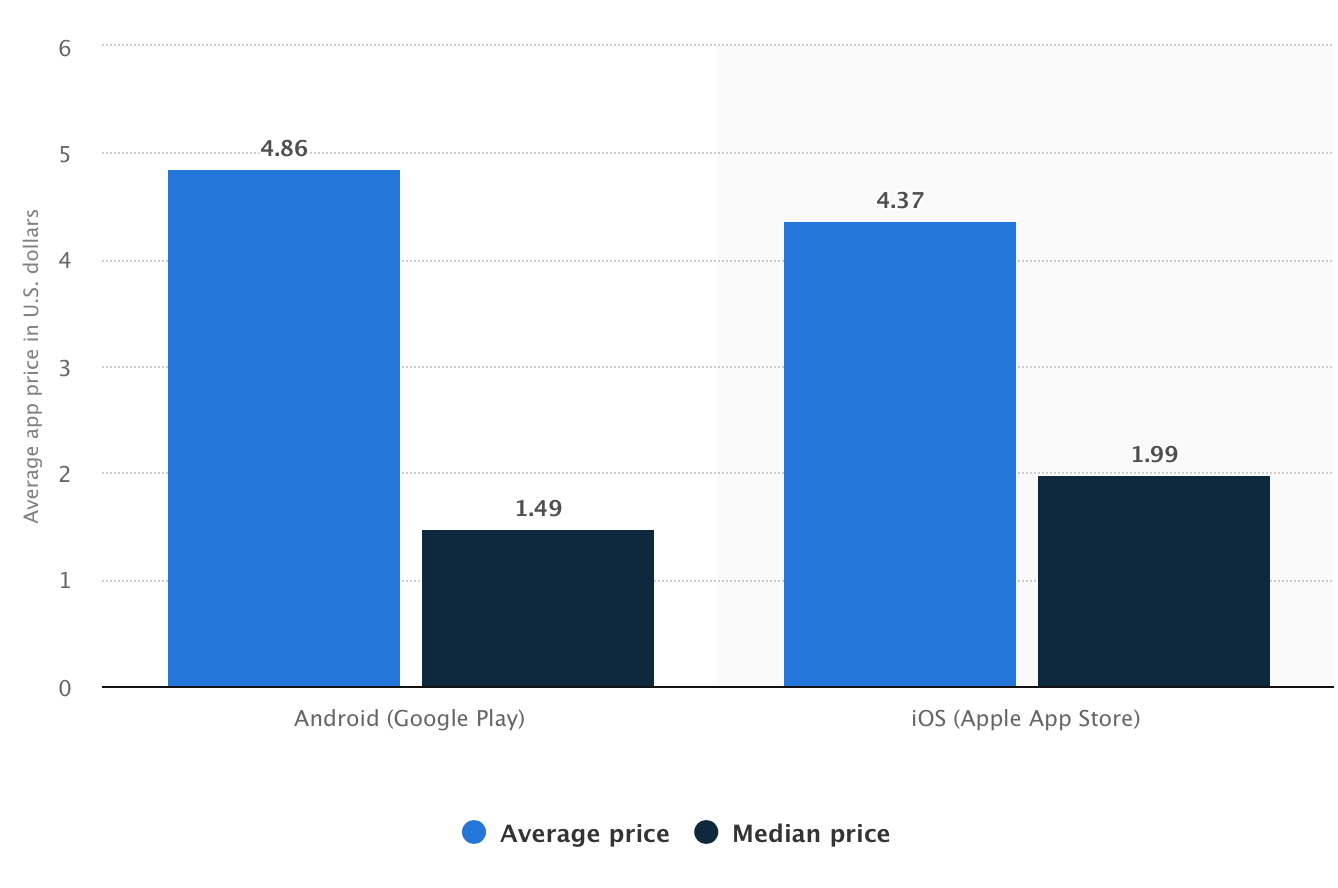
\includegraphics[keepaspectratio]{resources/images/image3.png}}

Quelle: statista, 2018

Spiele in App-Form für Tablet-Computer können in Zukunft eine größere
Zielgruppe erreichen, da vermutlich solche Hardware noch häufiger als
Spielkonsolen in den Haushalten vorhanden ist. Diese Geräte werden von
den Erwachsenen (Primärnutzer) zumeist zu Zwecken des erweiterten
Medienkonsum, also Zeitunglesen oder zum Videos schauen genutzt. Bei
hochwertigeren Angeboten im Bereich Spiele-App werden auch Preise im
niedrigen zweistelligen Bereich eingefordert. Diese Bepreisungen liegen
allerdings weit unter den Verkaufspreisen für aktuelle Vollpreistitel
für Spielkonsolen oder PC-Systeme. Diese Spiele schlagen mit
durchschnittlich 36 € zu Buche. Auf der nachfolgenden Abbildung 4.2 ist
in diesem Segment eine nahezu konstante Preisentwicklung zu sehen, die
entsprechende Hardware, also die Spielkonsolen, welche benötigt werden,
um diese Medien abzuspielen, weisen allerdings eine
Preissteigerungstendenz auf. Dies steht im Gegensatz zu den sinkenden
Kosten für Tablet-Computer.

Abb. 4.2: Durchschnittliche Spiele-Preise

\pandocbounded{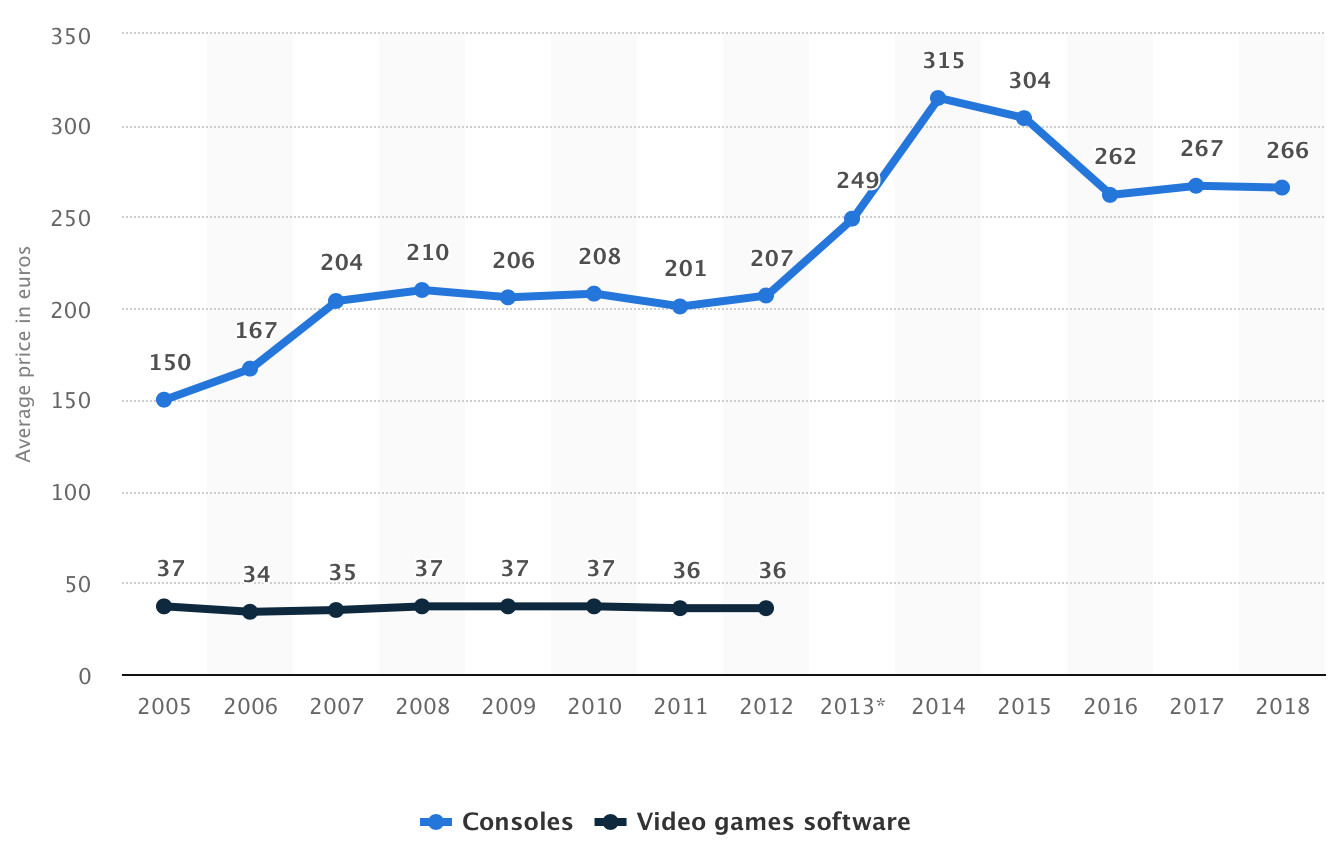
\includegraphics[keepaspectratio]{resources/images/image4.png}}

Quelle: statista, 2018

Nach Urlen (2017) sollen Kreativ-Apps für Kinder vorgezogen werden.
Diese Apps mit pädagogischer Eignung, sollten dem Autor zufolge
gemeinsam mit Freunden oder Eltern verwendet werden. Er verweist auf die
Spiele-App-Datenbank des Deutschen Jugendinstituts, die insbesondere
eine pädagogische Bewertung der Angebote ausschreibt. Holler (2012)
weist auf den Umstand hin, dass die Beurteilung der pädagogischen
Eignung von Medien, also der ‚Gebrauchswert`, aus Sicht der Kinder
getätigt werden muss. Diese Perspektive ist einzunehmen, um
nachvollziehen zu können, welche Einstellung ein Kind zu den Inhalten
einnimmt und welche persönlichen Rückschlüsse ein Kind daraus für sich
zieht. Auch konstatiert Holler, dass Kinder häufig aus den
Unterhaltungsmedien bekannte Figuren kennen und diese automatisch
positiv bewerten, um ihrer Peergroup anzugehören. Laut Urlen (2017) sind
keine pauschalen Aussagen über den Schaden oder Nutzen für Kinder von
App-Nutzung möglich, der Autor verweist an dieser Stelle darauf, dass
die Medienkompetenzschulung im Rahmen der elterlichen Erziehung und des
Vorlebens stattfinden sollte (Bundesjugendministerium, 2017).

Die WHO empfiehlt für Kinder unter zwei Jahren auf digitale Angebote zu
verzichten. Nach ihrer Einschätzung sind 80 \% der Minderjährigen zu
wenig körperlich aktiv. Im Alter ab zwei Jahren, sollten Kinder nur
unter der Betreuung der Eltern interaktive digitale Medien verwenden und
diese sollten insgesamt auf kurze Dauer begrenzt sein. Die Forschung
muss grundsätzlich noch klären, ab welcher Altersgruppe der Einsatz von
digitalen Medien Vorteile bringen kann und mit welchen Inhalten und
Spielmethoden Spiele versehen sein müssen, um keine nachteiligen
Auswirkungen auf die Kinder zu haben. Wie ein Spiel auf seine Nutzer
wirkt, ob der Spielende Freude daran hat und dauerhaft spielen wird, ist
maßgeblich durch das Gamedesign bestimmt (Strahringer \& Leyh, 2017).
Zum Beispiel sollte auch das Verlieren bzw. Scheitern an einer
Herausforderung Spaß machen oder anderweitig lohnenswert sein.
Andernfalls bestünde Frustrationsgefahr des Spielers und er verlöre
wohlmöglich die Lust am Weiterspielen. An dieser Stelle herrscht in der
gängigen Forschung Ungewissheit, ob heutige Angebote mit ihrem
Gamedesign die Entwicklung des Kindes optimal fördern.

Richtet man die Frage nach zukünftigen technologischen Innovationen
direkt an die besagte Zielgruppe, wie in einer Studie der Telekom mit
Zehn- bis Siebzehnjährigen, in deren Verlauf zukunftsorientierte
Prototypen konstruiert wurden, kamen diese Kernaussagen zusammen: 1.
Alles wird vernetzt sein, 2. Umgebungen werden intelligent, 3. Städte
reagieren auf individuelle Bedürfnisse, 4. Roboter vereinfachen das
Leben, 5. Digitale Kommunikation ist ins physische Leben eingebettet, 6.
Virtual \& Augmented Reality ist massentauglich, 7. Aktionen ersetzen
klassische User Interfaces (UI), 8. Biometrische Daten ersetzen
Passwörter, 9. Informationen werden vom Nutzer verwaltet und 10.
Technologie wird neue Verhaltensweisen erzeugen (von Reventlow \&
Thesen, 2019). Wie zuvor erwähnt, kann den sogenannten ‚Digital
Natives`, so wird die Generation, die von Klein an mit Mikrotechnologie
aufgewachsen sind, genannt, eine natürliche und organische Neigung zu
digitalen Erlebniswelten konstatiert werden. Um dieses Nutzungsverhalten
und das veränderte Lebensumfeld von Kindern zu erfassen, fasst das
Internationale Zentralinstitut für Jugend- und Bildungsfernsehen in
einer jährlich erscheinenden Studie mit dem Titel ‚Grunddaten Kinder und
Medien` dazu erhobene Daten zusammen. In dieser Studie geht hervor, dass
Kinder auf dem Tablet-Computer zu allermeist Spiele spielen, dicht
gefolgt von der Nutzung des Internets. Kinder spielen zu 75 \% zumindest
selten auf ihrem Tablet, in dieser Gruppe jedoch häufiger regelmäßig
oder oft. Die Smartphone-Nutzung bei Zehn- und Elfjährigen stieg von
2014 auf 2017 von 71 \% auf 87 \%, die Tablet-Nutzung in dieser
Altersgruppe sogar von 39 \% auf 61 \% (IZI, 2019). Diese Analyse
schlägt sich insbesondere auch in der aktuellen Neuorientierung der
Industrie hin zu dieser Zielgruppe und der entsprechenden Gerätegruppe
(mobile Endgeräte) nieder.

Das übergeordnete Ziel der BenBox.org ist Edukation. Die Festlegung des
Titel auf den Bereich der Gesundheitsförderung liegt insbesondere
wirtschaftlichen Betrachtungen zu Grunde. Der Gesundheitsmarkt ist ein
sehr wachstumsstarker Markt, bietet Förderungen durch die GKV und
erfreut sich hoher Beliebtheitsgrade. Ein eHealth Produkt muss sich
allerdings den Anfordernissen der Nutzer bzw. Patienten im
Gesundheitsmarkt, sprich der Volksgesundheit stellen. Im Jahre 2015 gab
es in den bekannten App-Stores über 100.000 Apps zu den Themen
Gesundheit und Medizin (Strotbaum \& Reiß, 2017). Nach Häckl (2010) wird
dieser Markt bis zum Jahr 2020 durchschnittlich um 5 \% pro Jahr
steigen, die Telemedizin- und Homecare-Sparte sogar um 10 \%.
Einhergehend mit diesen Erhebungen rechnet die Europäische Kommission,
dass der eHealth Markt in Europa, mit einem derzeitigen Anteil von
ungefähr 2 \% der Gesundheitsausgaben, fast halb so finanzstark wie der
Pharmamarkt wird. Zahlreiche Aussagen von Experten im Gesundheitswesen
(Leistungsanbieter, Kostenträger, Organisationen, Industrie) bestätigen
diese Prognosen. So gaben nach Häckl (2010) in einer Studie 80 \% der
befragten Technologie-Anbieter an, dass in diesem Bereich ein
Umsatzwachstum zu erwarten sei, 73 \% der in der Studie befragten
Leistungsanbieter sehen Deutschland im eHealth-Sektor als einen
wichtigen Standort an. In der Gliederung der Europäischen Kommission ist
folgende Aufteilung des Marktes zu finden:

\begin{enumerate}
\def\labelenumi{\arabic{enumi}.}
\tightlist
\item
  Klinische Informationssysteme
\item
  Telemedizin und Homecare
\item
  Integrierte (regionale / nationale) Gesundheitsinformationsnetzwerke
\end{enumerate}

4. Systeme zur Unterstützung des Gesundheitswesens (keine direkte
klinische Anwendung, z.B. Gesundheitserziehung)

Das dieser Arbeit zu Grunde liegende Produkt ist somit der 4. Kategorie
zuzuordnen.

\textbf{4.1 Serious Game in der Edukation (eLearning)}

Der bildende Ansatz des BenBox.org Serious Games enthält mit den Punkten
‚Edukation` und ‚Gesundheitsförderung` eine Zweigliederung. Die
Edukation soll im Spielverlauf durch eine Auseinandersetzung mit
Geschichts-, Religions- und Informationstechnologiewissenschaften
stattfinden. Im Speziellen werden die Geschichts- und Religionsbezüge
durch die Expansionspolitik des Römischen Reiches sowie der katholischen
Kirche thematisiert. Das Kinder spielerisch nicht nur motorisch lernen,
ist nach Spitzer (2002) ein unbestrittener Fakt. Er konstatiert, dass im
Vergleich zu anderen Arten, beim Menschen die Betonung auf dem (fit)
Werden liegt, nicht so sehr auf dem ‚fit sein von Anfang an`. Dies soll
größere Potentiale im späteren Verlauf der Gehirnentwicklung bieten. So
kann davon ausgegangen werden, dass auch ein Kind auf vielen
verschiedenen Ebenen lernt und eine Limitierung einer App auf nur eine
Lernebene (z.B. Motorik) nicht nötig, evtl. auch gar nicht sinnvoll ist.
Die BenBox.org Erzählung knüpft an diese neurowissenschaftlichen
Sachverhalte an und projiziert besagte Entwicklungspotentiale des
menschlichen Gehirns auf die beiden Roboter des Spiels. Zuerst beginnt
die Erzählung mit neuem Leben, in Form der Inbetriebnahme der Roboter.
Diese stehen sinnbildlich für das Aufwachsen des Kindes und später auch
für das eigentliche Menschwerden. Roboter werden von Kindern überwiegend
positiv bewertet und üben häufig eine große Faszination auf diese
Zielgruppe aus (Reventlow \& Thesen, 2019). Am Anfang des Spieles steht
der Körper im Vordergrund, also das dingliche Erleben, welches mittels
motorischer Übungen erfahren wird. Eltern sind laut Daun (2012) allein
verantwortlich für die Entwicklung ihres Kindes, auch wenn sie die
Verantwortung bei steigendem Alter ihres Kindes häufig aufteilen. Das
komplexe Thema der Erziehung kann der Autorin nach, durch Hilfe von
Fachleuten oder Angeboten unterstützt werden.

Im weiteren Spielverlauf der BenBox.org findet mehr und mehr eine
Auseinandersetzung mit geistig-spirituellen Inhalten statt, im
Spielgeschehen z.B. versinnbildlicht mit der Programmierung der Roboter.
Nach dem Psychologen und Philosophen William James teilt sich der Mensch
in ein körperliches, mentales und spirituelles Selbst. Neben den
motorisch-koordinativen Inhalten wird im Spiel eben auch eine
Betrachtung der spirituellen und kulturellen Belange des Menschen bzw.
Kindes vollzogen. Nach Bourdieu (1983) gibt es ein kulturelles Kapital,
mit dem der französische Soziologe das Wissen um Dinge wie Kunst,
Kulturgüter und Geschichte meint. Kinder und Erwachsene, die in diesen
Bereichen gebildet sind, erschließen sich häufig eine höhere
(berufliche) Entwicklung (Jæger \& Karlson, 2018). Der Kritik nach dem
übermäßigen Einsatz der digitalen Techniken widerspricht Krämer (2019)
und weist auf die Wichtigkeit von formatierten Flächen hin. Die
Philosophin an der Freien Universität Berlin gibt zu bedenken, dass alle
Wissenschaften, technisch-architektonische Arbeiten und die
gesellschaftliche Kommunikation undenkbar wären, ohne die Erfindung von
Papier und Stift, heute abgelöst durch z.B. Tablet-Computer. Die Autorin
verweist bei Nutzung digitaler Inhalte allerdings auf die Schrumpfung
des Intervalls zwischen Lesen und Verstehen hin, dem ihrer Aussage
zufolge das kritische Denken und die Einsicht entspringen. So auch
Goldin und Kutarna (2016), die anmahnen, dass die Kommunikation mittels
der modernen Medien nicht immer auf Fakten beruhe. Laut den Autoren soll
das Schlüsselelement für die Renaissance, also der Zeit des großen
Aufschwungs in Kunst, Kultur und Technik, maßgeblich der Buchdruck von
Gutenberg gewesen sein. Bei der Betrachtung der neuen Technologien
sprechen sie sogar von der zweiten Renaissance, in welcher sich die
Menschheit zurzeit befindet. So kann das Medium Serious Game sicherlich
als Wissensvermittler in der Altersgruppe Kinder und Jugendliche
fungieren. Als Beispiel dieser Wissensvermittlung sei auf die
Thematisierung der Reliquienverehrung im BenBox.org Prototypen
verwiesen. Dieses Thema wird im Spiel zentral behandelt und dem Spieler
erklärt, dass die Stadt Köln so zu Reichtum und Ansehen gelangt ist.
Nach Legner (1989) kann dieses Ritual als der Versuch angesehen werden,
den Toten wieder lebendig zu machen. Durch Zurschaustellung und Anbetung
von Gebeinen erreichten religiöse Menschen Linderung ihrer Leiden. Diese
Tatsachen sollen den spielenden Kindern erklärt und veranschaulicht
werden und seinem kulturellen Kapital als Wissen hinzugefügt werden. Da
die menschliche Zivilisation maßgeblich von der Durchführung von
religiösen Ritualen und Praktiken geprägt wurde, kann von einer
gleichbleibend hohen Relevanz dieses Themas ausgegangen werden (Gugutzer
\& Staack, 2015). An den hohen Kirchenaustritten, insbesondere aufgrund
von Skandalen, lässt sich jedoch der allgemeine Bedeutungsverlust der
Kirche im 21. Jahrhundert erkennen. Das Meinungsforschungsinstitut Forsa
ermittelte 2015 in einer Umfrage, dass 61 \% der Deutschen Religion und
Glaube keine oder nur noch eine geringe Bedeutung zu räumen. Im Spiel
wird mittels der Themen Religion und Spiritualität, die im Alltag bei
den meisten Familien keine Bedeutung mehr zu haben scheinen, das
kulturelle Erbe der Menschheit in den Erzählstrang eingearbeitet und
thematisiert. Dies geschieht nicht zuletzt auch wegen der erzählerischen
und philosophischen Möglichkeiten, die diese Themen bieten.

Die Story spielt in einer Science-Fiction-Parallelwelt, was größte
erzählerische Freiheiten gewährt und findet zum heutigen Zeitpunkt
statt. Der Comic- und Erzählstil ist beschreibbar als eine Mischung aus
der Nickelodeon (Privater Fernsehsender für Kinder) Kindersendung ‚The
Rugrats` und dem Sci-Fi-Comic ‚Futurama` von Matt Groening (Erfinder der
Simpsons-Serie). Der Storyverlauf setzt seinen Fokus auf die Spätantike
und Frühes Mittelalter mit dem Schwerpunkt auf der Romanik, dem
Römischen Reich sowie der katholischen Kirche und führt die Spieler in
Außeneinsätzen auf der ‚Via Sacra` überwiegend in solche historischen
Bauwerke. Die Romanik ist die erste ganz Europa umfassende Epoche
mittelalterlicher Kunst und in Köln augenscheinlich durch die ‚Via
Sacra` mit den zwölf Groß-Romanischen Kirchen als christliche
Sakralkunst zu begreifen (Toman, 1996). Somit kann das Spiel mit dem Dom
als Identifikationsobjekt, gerade im Kölner, aber auch deutschsprachigen
Raum, auf eine hohe Wiedererkennungsrate hoffen. Die BenBox.org
Geschichte ist als ein pseudo-wissenschaftlicher Geschichts- und
Religionsdiskurs zu verstehen und soll den Kindern Gedankenanstöße
insbesondere zu religiösen, spirituellen und philosophischen Themen
geben. Was unter diesen Begriffen im Rahmen dieser Arbeit zu verstehen
ist, soll zuvor in kompakter Weise definiert werden. Religion steht in
der BenBox.org Erzählung für die Auseinandersetzung mit dem
Unbegreiflichen, dem was man nicht wissen kann oder darf. Außerdem stand
die Religion immer unter der Deutungshoheit der katholischen Kirche, was
sich z.B. in den christlichen Dogmen ersehen lässt. Religion bekommt
heutzutage daher den Anstrich des Althergebrachten, des Verstaubten und
scheint geradezu nicht mehr mit der Moderne zu vereinbaren zu sein (Lay,
1995). Der Spieler wird häufig in Kirchen geführt und erfährt dort
vielfältiges historisches und religiöses Wissen. Dort gerät er in
unmittelbare Gefahr als er den ‚Kleaner` Robotern begegnet und wird
somit mit der eigenen Sterblichkeit konfrontiert. Dieses unausweichliche
Ende der menschlichen Existenz wird in Form der Reliquien greifbar
gemacht. Da gerade der Tod schon immer der Deutungshoheit der Kirche
oblag, wird dieses Thema im Spiel durch den Blick der Religion
betrachtet und diskutiert und wenn nötig, werden die Erklärungsmodelle
der kirchlichen Dogmen verworfen. Der Begriff Spiritualität hat nach
Bucher (2014) den Umhang des Mittelalters abgelegt und wird heutzutage
quasi inflationär benutzt. Er beschreibt im Spiel das Immaterielle,
steht sowohl auch für das Phantastische und wird gleichzeitig bei den
inhaltlichen Bezügen zur Mythologie verwendet. Demgegenüber steht die
philosophische Auseinandersetzung für die wertfreie Betrachtung eben
solcher Sachverhalte, worin die BenBox.org Erzählung sich verpflichtet
fühlt.

Die BenBox.org Science-Fiction-Story wird den Kindern außerdem
IT-Begriffe und Kenntnisse in einfacher und plastischer Weise erläutern.
Die Sachverhalte werden im Schwerpunkt Technologien sein, mit denen die
Kinder in Zukunft in Berührung kommen werden, allerdings auch
gegenwärtige IT-Produkte. Eine nicht abschließende Aufzählung von IT
Begriffen, vorrangführt von dem BenBox.org Spielelement, das diese
Technologie verkörpert: ‚BenBox` ≙ Starke KI, ‚SAM` und ‚SEB` ≙ Roboter,
‚STRIX` ≙ Updates und die ‚BenBox Protokolle` ≙ Datenschutz. Die
IT-Landschaft wird immer komplexer und kann von einem einzelnen kaum
noch überschaut werden. Assistenz-Systeme wie Google Assistent, Siri
(Apple) und Alexa (Amazon) versprechen daher Erleichterung im Alltag und
bündeln in geschlossenen System die verfügbaren Funktionen. Gerade der
Konsum, also der Kauf von Produkten, steht im Vordergrund. In
Unternehmen erlauben programmierte Chat Bots eine Optimierung der
Geschäftsprozesse. Daten werden verschlüsselt in der Cloud gespeichert,
der Gesundheitsmarkt z.B. erfordert den verstärkten Einsatz von
Sicherheits- und Datenschutztechnologien, um Daten zu erfassen, zu
speichern und zu verarbeiten. Deep Learning Technologien vermögen es
sogar, Aufgaben, die im Grunde für den Menschen leicht sind, für ein
Computersystem jedoch schwer zugänglich, da nicht durch mathematische
Formeln berechenbar, Muster zu erkennen, wie z.B. Sprache oder Gesichter
(Nvidia, o. J.). Daraus kann in Zukunft eine starke KI entstehen, sobald
sie verschiedene Lösungsansätze gegeneinander abwiegen kann. Im Spiel
werden die erwähnten Begriffe und Sachverhalte aufgegriffen und dem
Spieler in interaktiver und symbolischer Form präsentiert. Der
zunehmenden Bedeutung von KI, wird im Spiel durch die BenBox im
Mittelpunkt Rechnung getragen. Die bildliche, linguistische und
interaktive Erfahrung des Spielers lässt hoffen, dass für ihn ein
nachhaltiges Lernen ermöglicht wird und aus pädagogischer Sicht eine
adäquate Vorbereitung auf die technologische Zukunft stattfindet.

\textbf{4.2 Serious Game in der Gesundheitsförderung (eHealth)}

Der Aspekt der Gesundheitsförderung des BenBox.org Serious Games umfasst
theoretische wie praktische Elemente. Wie im Einleitungsteil dieser
Arbeit formuliert, ist das Ziel von Angeboten im Genre Exergames das
Embodiment. Vereinfacht ausgedrückt kann dieser Begriff, welcher aus der
kognitiven Verhaltensforschung stammt, mit Bewusstsein in Beziehung zum
eigenem Körper verstanden werden. Diesen Ansatz machen sich die
somatopädagogischen Disziplinen zunutze und verwenden Techniken, die den
Schüler in die Lage versetzen, mehr aus seiner Körperlichkeit
abzuleiten, als er es sonst im hektischen Alltag zu leisten vermag. Nach
Steinmüller, Schaefer und Fortwängler (2009) erfordert das Abwegen von
Handlungsoptionen, wie zuvor bei der Entwicklung einer starken KI
beschrieben, im menschlichen Gehirn eine inhibitorische Leistung.
Andernfalls muss auf den ersten Reiz automatisiert reagiert werden und
ineffiziente Bewegungsmuster können das Ergebnis sein. Kindern im
Grundschulalter lastet zudem nicht selten ein unnatürlicher Sitzzwang
sprichwörtlich auf den ‚Schultern`, ob ein ergonomischer Schulranzen mit
digitalen Büchern, sogenannten eBooks (versprechen Gewichtsreduktion),
dem krummen Rücken Einhalt gebieten kann, mag zu bezweifeln sein. Aus
diesen Gründen werden im Spielverlauf vom Spieler real-motorische
Auseinandersetzung mit der ihn umgebenden räumlichen Dimension
abverlangt. ‚SAM` und ‚SEB`, die beiden Spielercharaktere, sind ganz wie
im Kindesalter aufgefordert, die einfachsten motorischen Übungen zu
absolvieren. Im Spielverlauf werden diese Aufgaben im ‚Holo Deck`
gezeigt und die Punkte vom jeweils anderen Spieler vergeben. Diese
Übungen werden immer fordernder und komplexer, die Kinder machen diese
motorischen Interventionen zum Teil mit Hilfsmitteln wie einem Balance
Board und Gegenständen wie einem Holzschwert und Schirm. Die gewonnen
Punkte werden im ‚Updater` vom Spieler durch die schwache KI ‚STRIX`
vergeben und auf die Fähigkeiten Beweglichkeit, Geschmeidigkeit und
Gleichgewicht verteilt. Diese Fähigkeiten werden dem Kind im
Spielverlauf erläutert und die Bezüge zum eigenen Körper aufgewiesen.

Nach Sinclair, Hingston und Masek (2009) und ihrer DualFlow Theorie,
muss ein solches Exergame die Balance zwischen spielbasierter
Herausforderung und der Spielerfähigkeit, sowie der Komplexität der
geforderten Bewegung und dem motorischen Fähigkeiten des Anwenders
herstellen. Nur dann wird ein immersives Erlebnis, sprich eine
Vertiefung in die virtuelle Welt stattfinden. Da die moderne Sensorik
von Unterhaltungsspielemedien kaum eine adäquate Bewertung von
Ganzkörperbewegungsmustern nach therapeutischen Gesichtspunkten erlaubt,
beginnen Deep-Learning-Ansätze unter größten Mitteleinsatz momentan
gerade erst Mimik zu erkennen, wird das BenBox.org Spiel zu zweit
gespielt. An den entsprechenden Stellen im Spiel wird ein Kind
aufgefordert eine Übung durchzuführen, während der Mitspieler diese
einschätzen soll. Hierbei wird strikt auf eine neutrale und
humanistische Bewertungsweise geachtet. Nach Daun (2012) liegen im Lob
bzw. der Kritik große Potentiale der Einflussnahme, aus pädagogischer
Perspektive jedoch auch in eine nachteilige Richtung. Frau Daun
beschreibt das Loben, wenn damit vom Lehrer gewünschtes Verhalten
gezielt aufgewertet wird, als emotionalen Aufladungstrick. Das führt auf
der neurobiologischen Ebene zu einer vermehrten Dopamin Produktion beim
Kind und nicht wie beim von Csikszentmihalyi beschriebenen ‚Flow`, zu
einer Noradrenalin und Serotonin Ausschüttung im Gehirn. Das Kind kann
nach Daun so seine natürliche Lernlust verlieren, wie in Abb. 4.2.1
schematisch skizziert.

Abb. 4.2.1: Angeborene Lernlust

\pandocbounded{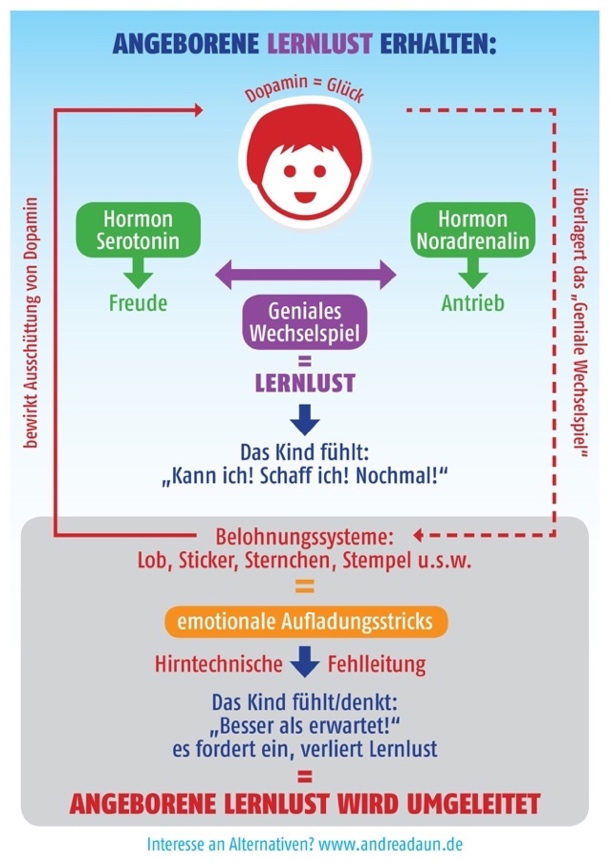
\includegraphics[keepaspectratio]{resources/images/image5.jpeg}}

Quelle: Andrea Daun, 2012

Letztendlich können die Transmittersysteme des Gehirns nicht isoliert
betrachtet werden, da nach aktuellen Erkenntnissen nie völlig
unabhängige Funktionen der Teilsysteme zu beobachten sind (Förstl,
2012). Daher ist die Aussage, dass nach Gaschler (2019) Jugendliche am
stärksten auf Lob reagieren an dieser Stelle bedeutsamer, als welche
Transmittersysteme an diesem Prozess beteiligt sind. Gaschler räumt der
Phase der Adoleszenz, präzise dem Alter von zehn bis neunzehn Jahren,
die ständige Verbesserung der Fähigkeiten Selbstbeherrschung und
Introspektion zu, gepaart allerdings mit Sensationslust, starker
Orientierung an den Gleichaltrigen und Risikobereitschaft. Im Besonderen
ist der Peer-Effekt ein Merkmal dieses Alters. Folglich kann davon
ausgegangen werden, dass die gegenseitige Bewertung gruppentypisches
Verhalten positiv bewertet und anders herum, untypisches Verhalten
schlechter. Dem gegenüber steht, gerade da häufig das Emotionssystem
meist vor dem Präfrontalkortex ausgereift ist, die leidenschaftliche und
kreative Auseinandersetzung mit Problemen. Die jungen Menschen sind
bereit altanerkannte Strategien beiseite zu legen, um neuen Ansätzen zu
folgen oder diese zu initiieren. Gerade diesen Umstand, das Erkunden von
neuen Lösungsstrategien, möchte die BenBox.org durch die Bewertung der
Mitspieler belohnt, gefördert und wertgeschätzt wissen. Im
Wirtschaftsleben und im eHealth-Sektor wird diese Eigenschaft und
entsprechende Technologien Disruption genannt (Strotbaum \& Reiß, B
(2017). Ein Begriff der gehäuft im Zusammenhang mit den neuen digitalen
Medien verwendet wird.

Soll eine derartige disruptive Applikation bzw. eine die disruptives
Verhalten fördert erfolgreich vermarktet werden, muss zusammenfassend
gesagt werden, dass der Spieler ein forderndes, aber auch lohnendes
Erlebnis erfahren muss. Daraus leitet sich ab, dass der Anwender eine
persönliche Erweiterung der eigenen Fähigkeiten erfährt. Eine Verwendung
von Gamification (Lob) im Sinne der Kundenbindung und Erweiterung des
Absatzes muss den Mitteln der bestmöglichen Entwicklung des Kindes nach
geordnet sein. Nur so kann der Ansatz dem Anspruch genügen ‚pädagogisch
wertvoll` zu sein. Resümierend soll dieser Anspruch bedeuten, dem Kind
kulturelles Wissen, Religiosität und Philosophie nahe zu bringen und die
Souveränität im Umgang mit sich und der Welt zu fördern. Ein zu diesem
pädagogischen Modell fast gegensätzlich stehender Ansatz ist in der
klassischen Werbung zu finden. Diese bedient sich Beobachtungen, wie der
Mensch auf bestimmte Situationen emotional reagiert. Häufig entstammen
diese Erkenntnisse der (klinischen) Psychologie. Als Beispiel wird ein
In-App-Kauf angenommen. Dieser Kauf bedeutet einen geringen Involvement
vom Nutzer und wird durch die primär emotionale Reaktion, die als eine
Art Vorentscheidung zuvor stattfindet, ausgelöst. Die sich erst
anschließende sekundäre, sachliche Bewertung, muss sich alsdann bei
einem Kleinstbetragkauf im Falle der Negativbewertung über eine starke
Emotion hinwegsetzen (Kroeber-Riel, \& Esch, 2015). Erfahrungsgemäß
zeigen Kinder, man stelle sich eine Mutter mit Kind an der Kasse eines
Supermarktes vor, an welcher Süßigkeiten, Spielkarten und dergleichen
dargeboten werden, hier wenig rationales Verhalten. Die Mutter spiegelt
in diesem Falle die rationale Bewertung dar.

Schwerpunkt des Produktes soll nicht allein auf der motorischen
Lernebene liegen, dann könnte man von einem klassischen Exergame
sprechen, von denen vielfältige Ausprägungen am Markt verfügbar sind.
Das Spiel soll vielmehr ein Produkt der allgemeinen Gesundheitsförderung
und Persönlichkeitsentwicklung sein. Nach Förstl (2012) umfasst die
Entwicklung des menschlichen Gehirns sowohl bio-psychische als auch
spirituelle Dimensionen. Letztere sind ein wesentlicher Bestandteil
menschlichen Erlebens, ist er doch ein narratives Wesen, das seine
Lebensgeschichte tagtäglich neuschreibt und im Kontext seiner aktuellen
persönlichen Wahrheit und Weltsicht immer wieder umdefiniert. Nicht
zuletzt dient das spirituelle Selbst der effektiven Auseinandersetzung
mit Krisen und Traumata. Gerade Traumata sind insbesondere in den
Bewegungs- und Haltungsmustern von Menschen abgebildet (Steinmüller,
Schaefer \& Fortwängler, 2009). Somatopädagogische Methoden erlauben
neben der Diagnose eben auch die therapeutische Intervention zur Lösung
dies gearteter Blockaden. Zuerst muss jedoch die Notwendigkeit einer
Veränderung erkannt und somit die Sinnhaftigkeit von ganzheitlicher
Heilung anerkannt werden. Die BenBox.org Erzählung deckt zu diesem
Zwecke einen Teil der geschichtlichen Tragödien in symbolischer und
kindgerechter Form auf. So soll dem Spieler ein Bewusstsein geschaffen
werden, dass er Teil einer transgenerationalen Geschichte ist. Auf diese
Weise kann das Kind Bezüge zur heutigen Gesellschaft mit ihren
unterschiedlichen Befindlichkeiten und Bedürfnissen aufstellen.

Da das Raumschiff in der Erzählung, es ist ein liegender Korpus, an den
menschlichen Körper erinnert, können neben motorisch-erzieherischen
Inhalten auch medizinische Zusammenhänge spielerisch bearbeitet werden.
Im ‚Maschinenraum` treibt quasi ein Herz das Sternenschiff an und
erlaubt damit Vergleiche zum Herz-Kreislaufsystem, so die Gänge des
Schiffes wie Blutgefäße des menschlichen Körpers anmuten. Infolgedessen
entsteht im Spielverlauf regelmäßig der Auftrag, die Systeme der ‚Pulp`
(engl. Fleisch), so heißt das Raumschiff, auf dem die Crew in das
irdische Sonnensystem gereist ist, zu reparieren, auf die Geschichte
übertragen also zu heilen. Diese Heilung findet indes auch im
Betriebssystem des Schiffes, sprich in der Programmierung statt. Im
BenBox.org Erzählstrang haben die Vorbesitzer des Schiffes an diesem
Modifikationen vorgenommen, was eine De-Programmierung von Nöten macht.
Diese und weitere Spielgeschehnisse finden im ‚Hangar` statt, wo auch
die ‚BenBox` (KI) anzufinden ist. Mittels der KI kann die Übertragung
vom Schiffs-Betriebssystem zum menschlichen Gehirn vollzogen werden und
den Kindern so die komplexe menschliche Neurobiologie vereinfacht
erläutert werden. In Feldenkrais (somatopädagogische Methode) ist hier
auch von Reorganisation im Sinne der ‚sensorischen Integration` die
Rede, an welcher insbesondere die somatomotorische Rinde des Großhirnes
beteiligt ist. Der Bezug zur menschlichen Motorik wird an dieser Stelle
ebenso vollzogen. Nach Schellhammer (2002) übernimmt diese
Schaltzentrale im Großhirn funktionale Aufgaben wie die Propriozeption
(Tiefenwahrnehmung). Diese motorischen Kerne, in denen komplexe
Bewegungsprogramme geplant und angebahnt werden können, sind dem
Hirnstamm übergeordnet. Phylogenetisch ist das propriozeptive System am
jüngsten, weist dadurch weniger stark ausgeprägte Kontakte zu den
anderen Systemen auf. Aufgrund der immer größer werdenden Extremitäten
des Menschen, welche der Hirnstamm, wegen der wachsenden
Ansteuerungskomplexität, nicht mehr in der Lage war zu steuern,
entwickelten sich Regionen im Großhirn die diese Aufgaben übernahmen
(Schellhammer, 2002). Auf die Motorik bezogen, spricht man an dieser
Stelle von kinästhetischer Differenzierungsfähigkeit. Differenziert
werden muss zwischen Kraft, Zeit und Raum. Die Kinästhetische
Differenzierungsfähigkeit ist eine wesentliche Komponente in der
modernen Rückenschule (Flothow, Kempf, Kuhnt \& Lehmann, 2011).
Insbesondere die Methode der Alexander-Technik, mit ihrem Kernthema
‚Bewusste Steuerung`, ist dazu geeignet den Schüler darin zu schulen,
mittels Hemmung von Reaktionsmustern (Inhibition), Bewegungsmuster
effizienter zu gestalten, in dem muskuläre Verspannungen gelöst werden
(Gaschler, 2019; Steinmüller, Schaefer \& Fortwängler, 2009). So kann
dieses gewichtige Thema der menschlichen Motorik spielerisch auf der
theoretischen und praktischen Ebene vermittelt werden und gilt als
Schwerpunkt des BenBox.org Exergames.

\textbf{4.3 Ökonomische Betrachtungen eines Serious Games}

Der Prototyp wurde von Kindern zwischen acht und neun Jahren gespielt.
Die Zielgruppe soll erweitert auf die Altersgruppe von Sechs- bis
Dreizehnjährige angesetzt werden. Nach Pyka (2017) sind junge Menschen
für das Marketing eine sehr sinnvolle Zielgruppe. Es gab 2014 laut einem
Bericht des Bevölkerungsfonds der Vereinten Nationen (UNPFA) rund
1,8~Milliarden Menschen im Alter von 10 bis 24, so viele wie nie zuvor
in der Menschheitsgeschichte, und ihre Zahl soll weiter steigen. Nach
Strotbaum und Reiß (2017) können gerade spielerische und motivierende
Ansätze, sprich Serious Games und Anwendungen mit Gamificationelementen,
im Präventionsbereich vielversprechend vermarktet werden. Die Autoren
konstatieren eine Hinwendung von bestehenden IT Unternehmen im
Gesundheitsmarkt zu diesem Thema, sowie Gründungen von Start-Ups in
diesem Bereich. Nun soll im Speziellen geprüft werden, ob ein Serious
Game ökonomisch Erfolg versprechend sein kann und wenn ja, unter welchen
Bedingungen dieser Erfolg erreicht werden kann. Um mit einer
Unternehmung erfolgreich zu sein, muss zuerst ein Produkt konzeptioniert
sein, um anschließend die Zielgruppe klar einzugrenzen. Nach Greiner,
Schulenburg \& Vauth (2008) ist eine Unternehmung im Gesundheitsbereich
in zwei Teile zu spalten - den Leistungsbereich und den Finanzbereich.
An der Wertschöpfung sind, wie im folgenden Schaubild (Abb. 4.3.1) zu
sehen, die Input Faktoren, die Erstellung, die Verwertung und der Output
beteiligt.

Abb. 4.3.1: Produktion von Gesundheitsprodukten

\pandocbounded{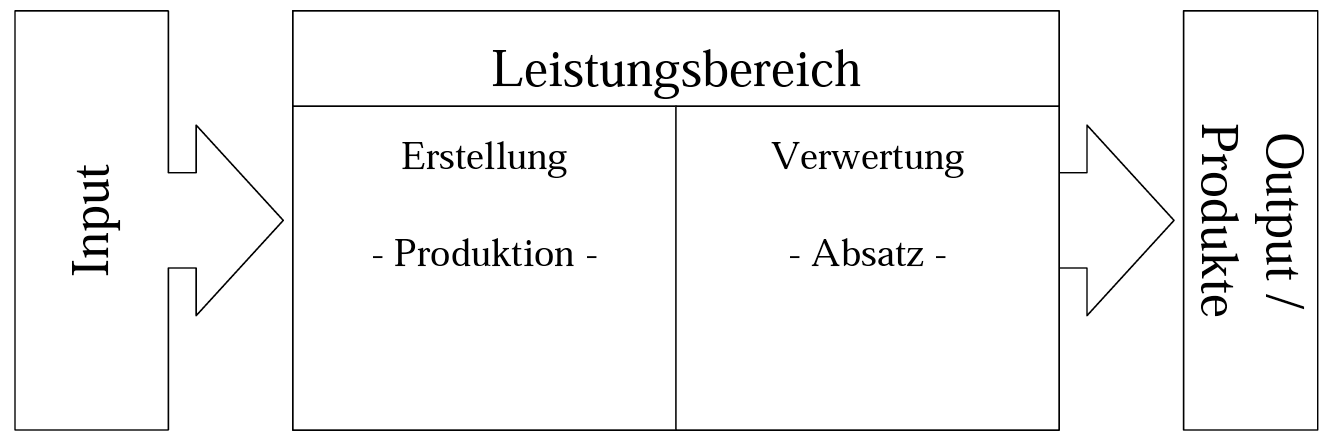
\includegraphics[keepaspectratio]{resources/images/image6.png}}

Quelle: Greiner, Schulenburg \& Vauth, 2008

Die Input Faktoren sind die Fähigkeiten des Entwicklers, sein
spezifisches Gesundheitswissen und die Fähigkeit kreative Anwendungen zu
konzeptionieren. Die Erstellung findet beim vorgestellten Produkt
hauptsächlich digital statt. Dazu wird ein Computer verwendet, um die
Programmierung durchzuführen, sowie um die grafischen Medien zu
erstellen. Hinzu kommen Auftragsarbeiten von zwei Zeichnerinnen. Als
fertiges Produkt (Output) entsteht der BenBen.org Prototyp.

Nun gilt es zu klären, welche Finanzierungs- und Vertriebswege für die
BenBox.org am sinnvollsten sind. Laut Strotbaum und Reiß (2017) muss
medizinische Expertise mit Kompetenz in der Softwaregestaltung verbunden
werden. Beispiele wie Freeletics zeigen, dass ein Unternehmen diese
Expertisen durch Mitarbeitergenerierung auch hinzuholen kann, um
erfolgreich zu sein kann. Die drei Gründer verkauften 2018 ihre Anteile
an der besagten Fitness-App in hoher zweistelliger Millionenhöhe, obwohl
die drei Betriebswirte über keinerlei medizinische Ausbildung verfügten,
geschweige denn Informatiker waren (Tischer, 2018). Ob dieses
Unternehmensmodell für die Anforderungen von qualitativen
eHealth-Lösungen am besten geeignet ist, soll an dieser Stelle nicht der
eingehenden Betrachtung unterzogen werden. Vielmehr soll aufgezeigt
werden, dass innovative digitale Produkte und nicht zuletzt Ansätze mit
unterhaltenden Charakter (Games, Serious Games etc.), im wachsenden
Markt große finanzielle Erfolge erreichen können. Dies sieht
mittlerweile auch die Bundesregierung so und veranschlagt 50 Millionen
Euro für das erste Jahr als Förderung von Spieleentwicklungen in
Deutschland. Dieses Geld soll im Bundeshaushalt 2019 freigegeben werden
und zur Förderung von Prototyp- und Produktion-Entwicklungen mit einer
Summe zwischen 30.000 bis 400.000 € ausgeschrieben sein (game - Verband
der deutschen Games-Branche, 2018). Auch Google, mit dem dazugehörigen
Mutterkonzern Alphabet, plant seine Bestrebungen im
Computer-Spiele-Markt auszubauen. Im Herbst diesen Jahres wird der
eigene Spiele-Streaming-Dienst Stadia erscheinen. Auf den Servern von
Google werden moderne Spiele gerendert und als interaktiver Inhalt auf
die Rechner der Kunden gestreamt. Stadia visiert einen großen Markt an
Gelegenheitsspielern an, denen die Anschaffung von spielefähiger
Hardware (Spielkonsolen und PC) zu teuer ist. Diese Zielgruppe kann mit
Googles Streaming-Dienst, per monatlicher Zahlung von 10 €, Zugang zu
vielen verschiedenen Spielen bekommen, wenngleich Vollpreis-Spiele noch
zusätzlich durch Einmalzahlungen erworben werden müssen (Herbig, 2019).
Der Vorteil ist, dass das Streaming von aufwendigen grafischen Szenen
vom Nutzer keine spezielle Hardware erfordert und somit auch auf
Rechnern in Schulen und Firmen zu Verfügung steht. Einzig die
Internetanbindung muss ein performanter Breitbandanschluss sein. Die
Game-Engine Unity, mit der viele hochwertige Spiele auch als
Crossplattform-Lösung entwickelt werden, ermöglicht die kostengünstige
zeitgleiche Entwicklung für mehrere Zielsysteme (PC, Konsole, mobile
Endgeräte etc.). Unity wird zum Start von Stadia diese
Streaming-Technologie von Google unterstützen. Auch unterstützt die
Game-Engine die Verwendung von VR-Brillen und ist mit allen am Markt
gängigen Technologien (HTC Vive, Oculus Rift etc.) kompatibel und bereit
auch diesen Wachstumsmarkt mit Angeboten zu adressieren.

\textbf{4.3.1 Vertriebswege}

Im Bereich der App-Spiele, die über App-Stores vertrieben werden, hat
sich mit Mikrotransaktionen oder In-App-Käufen eine neue
Monetarisierungsform etabliert. Diese versprechen große Einkünfte für
den Hersteller, da eine stetige Einnahmequelle generiert wird und nicht,
wie bei konventionellen Festpreistiteln üblich, nur eine einmalige
Gewinnausschüttung beim Kauf. Die In-App-Käufe bescheren dem Spieler
neue Spielinhalte, häufig sind das Spielgegenstände, die das Erreichen
des Spielzieles vereinfachen. 2016 legte der Verkauf dieser virtuellen
Güter um 17 \% zu, auf insgesamt 659 Millionen Euro im Bereich der
Free-to-Play Spiele, bei denen der Hersteller nur durch diese
Zusatzangebote Geld verdient, da das Spiel grundsätzlich umsonst ist.
Monatliche Investitionen der Nutzer sind auf 13,57 € gestiegen (game -
Verband der deutschen Games-Branche, 2017). Clash Royale, ein
kostenloses Handy- und Tablet-Spiel, konnte in den ersten zweieinhalb
Jahren über zwei Milliarden Euro umsetzen. Dazu verwenden die Hersteller
Machine-Learning-Technologien, mit denen die In-App-Angebote
maßgeschneidert für den einzelnen Spieler angepriesen werden (Heim,
2018). Auch Anbieter von klassischen Brettspielen reagieren auf die
Entwicklungen und verfolgen, durch die zusätzliche Implementation einer
Handy- oder Tablet-App in das Spielgeschehen, in einigen ihrer Angebote
einen hybriden Spielansatz. Nach Niebert (2018) sind diese Apps teils
kostenlos, teils kostenpflichtig und generieren zusätzliche
Spielinhalte, speichern den Spielstand und helfen bei der Auswertung.
Auch Apps, die die Spielregeln erklären sind am Markt verfügbar. Ob
diese zusätzlichen digitalen Applikationen zudem In-App-Kauf-Funktionen
implementierten haben, muss im Einzelfall geprüft werden.

Eine klassische Einnahmequelle für digitale Medien ist die Schaltung von
Werbung für Produkte von anderen Herstellern. Sogenannte ‚Rich-Media`
Formate zeigen komplexe Banner, auf denen Video, Audio sowie interaktive
Inhalte zu sehen und hören sind. Da die Klickrate (auf einen
Werbebanner) im Schnitt nur 0,09 \% entspricht, muss ein Werbetreibender
herausstechen, um seine Zielgruppe ohne Streuverluste zu erreichen
(Lammenett, 2014). Ein Anbieter der Werbefläche verkauft, profitiert je
nach Abrechnungssystem von erfolgreich vermarkteter Werbung seines
Kunden, sollte diese also gezielt einsetzen und dem Kunden gegenüber
seine Zielgruppe und deren Bedürfnisse detailliert beschreiben können.
Für ein Serious Game für Kinder sollte die Werbung also z.B. Spielzeug,
aber auch weitere digitale Angebote wie kindgerechte Spiele und Videos
enthalten. Somit kann ein Spieleanbieter auch ohne In-App-Verkaufssystem
Umsatz generieren. Der Entwickler Part Time Monkey Oy verzeichnete für
das Spiel Breakout Ninja, nachdem Apple das Spiel in der Kategorie
‚neues Lieblingsspiel` ausgezeichnet hatte, mehr als 650.000 Downloads.
Part Time Monkey Oy nahm in dieser Zeit jedoch nur etwa 1.000 € durch
den In-App-Kauf zum Deaktivieren der Werbung ein, in einer Woche jedoch
rund 21.500 € für Werbung (Schneider, 2017). Apple verdient aus
In-App-Käufen generierten Zahlungen zu 30 \% des Umsatzes mit. Diese
Regelung trifft auch große Software-Anbieter, wie zum Beispiel Microsoft
mit ihren Office-Programmen, die ihre Programme über den Apple App-Store
verbreiten (Günther, 2014). Viele Spieleentwickler nehmen in ihren
aktuellen Angeboten jedoch Abstand von Mikrotransaktionen und Werbung,
weil sie grundsätzlich auf den Nutzer abschreckend wirken und verwenden
wieder Fixpreise für ihre Produkte (Beineke, 2019). Unter iOS (iPhone
und iPad-Geräte) lässt sich die In-App-Kauf-Funktion über die
Einstellung ‚Bildschirmzeit`, zum Schutz von Kindern, auch komplett
deaktivieren, damit kein unbeabsichtigter Kauf mehr stattfinden kann. Zu
denken gibt allerdings die Integration dieser Option an besagter Stelle
im Mobile-Betriebssystem von Apple, da die Rubrik ‚App-Store` ebenso in
den Einstellungen hinterlegt ist und diese Funktion dort sinngemäß zu
erwarten wäre. Auch ist die Deaktivierung von In-App-Käufen unter
‚Bildschirmzeit` nur möglich, wenn die Funktion aktiviert wird. Dies
legt die Vermutung nahe, dass Apple den Verlust von Einnahmen dadurch zu
kompensieren versucht, mehr Nutzer- bzw. Nutzungsdaten zu gewinnen.
Becker (2019) zufolge versucht Apple sich von seinen Mitbewerbern
(Microsoft, Google etc.) abzusetzen, indem sie insbesondere die
Datenschutz- und Privatsphäre-Ansprüche ihrer Nutzer respektieren und
dementsprechend Funktionen in ihre Produkte integrieren. Das Unternehmen
aus Cupertino in Kalifornien liefert im eigenen Apple App-Store für
Eltern einen detaillierten Leitfaden zu diesen Themen und beschreibt
dort die verfügbaren Schutzfunktionen für Kinder. Hier muss allerdings
grundsätzlich zwischen geschicktem Marketing und unternehmerischer
Realität unterschieden werden, wie das gezeigte Beispiel von Apple
aufzeigt. Laut Statista wurde 2011 mit diesen unterschiedlichen
Strategien pro Games-App-Nutzer auf dem Apple Betriebssystem iOS im
Durchschnitt ein Umsatz von 4 US-Dollar pro Monat erzielt.

\textbf{4.3.2 Finanzierungsstrategien}

Der ‚Calliope mini`, ein Mini-Computer mit dem Schüler ab der dritten
Klasse Programmieren lernen und ein Verständnis von Mikrotechnologie
bekommen, wird in vielen Schulen in Rahmen von Pilotprojekten
eingeführt, bisher finanziert durch Crowdfunding. In den einzelnen
Bundesländern haben Stiftungen zusätzlich Gelder zur Schulung des
Personals bereitgestellt. In Zukunft möchte die Calliope gGmbH die
‚Calliope mini Boards`, sowie die benötigten Schulungen, durch die
einzelnen Länder finanziert bekommen. Diese Finanzierungen würden im
Rahmen der Digitalisierungsstrategien der verschiedenen
Landesregierungen ermöglicht. Die Krankenkassen wiederum entwickeln
eigene Medizinprodukte oder fördern innovative eHealth Applikationen von
IT Unternehmen oder Start-Ups. Die Versicherten können dann diese Apps
und Spiele zu vergünstigten Konditionen oder im Rahmen der
Gesundheitsförderungen der jeweiligen GKVs nutzen.

Das Crowdfunding eine gute Möglichkeit für Spieleentwickler-Studios mit
keinem oder geringem Eigenkapital ist, zeigt das Beispiel von Cloud
Imperium Games. Gründer, Hauptdesigner und Erfinder der Weltraumkampf-
und Handelssimulation ‚Star Citizen`, Chris Roberts, der in der
Spieleszene einen guten Ruf angesichts seiner bekannten und
erfolgreichen Spiele in diesem Genre inne hat, sammelte über 222
Millionen US-Dollar durch Crowdfunding ein. Allerdings steht Roberts in
der Kritik diese Investitionen zu verschwenden - er verzichtet auf den
Vertrieb durch einen Spiele-Publisher und trifft alle Termin- und
Designentscheidungen ohne Kontrollinstanz selbstverantwortlich. Kritiker
behaupten, klare Beweise dafür zu haben, dass der Entwicklungsprozess
ineffizient und evtl. auch ineffektiv sei. Zusätzlich zu den Geldern
durch Privatkapitalgeber besorgte Roberts Fremdkapital von Banken.
Außerdem floss Geld durch Eigenkapital in das Unternehmen ein, dessen
Wert auf aktuell insgesamt eine halbe Milliarde US-Dollar geschätzt wird
(Bathge, 2019). Ein deutlich kleinerer Spieleentwickler verfolgte für
Episode 1 seines Spieles ‚Bolt Riley` eine zweiteilige
Crowdfunding-Strategie und veröffentlichte sein Projekt auf zwei
verschiedenen Crowdfunding Plattformen mit dem Gesamtziel von 64.000
US-Dollar. Sein Budgetplan, wie in Abb. 4.3.2.1 zu sehen, zeigt die
Hauptausgaben Programmierung, Vertonung der Protagonisten und
musikalische Untermalung, deren Kosten mit zusammen 70 \% des
Gesamtinvestitionsvolumens veranschlagt sind.

Abb. 4.3.2.1: Budgetplan ‚Bolt Riley Episode
1`\pandocbounded{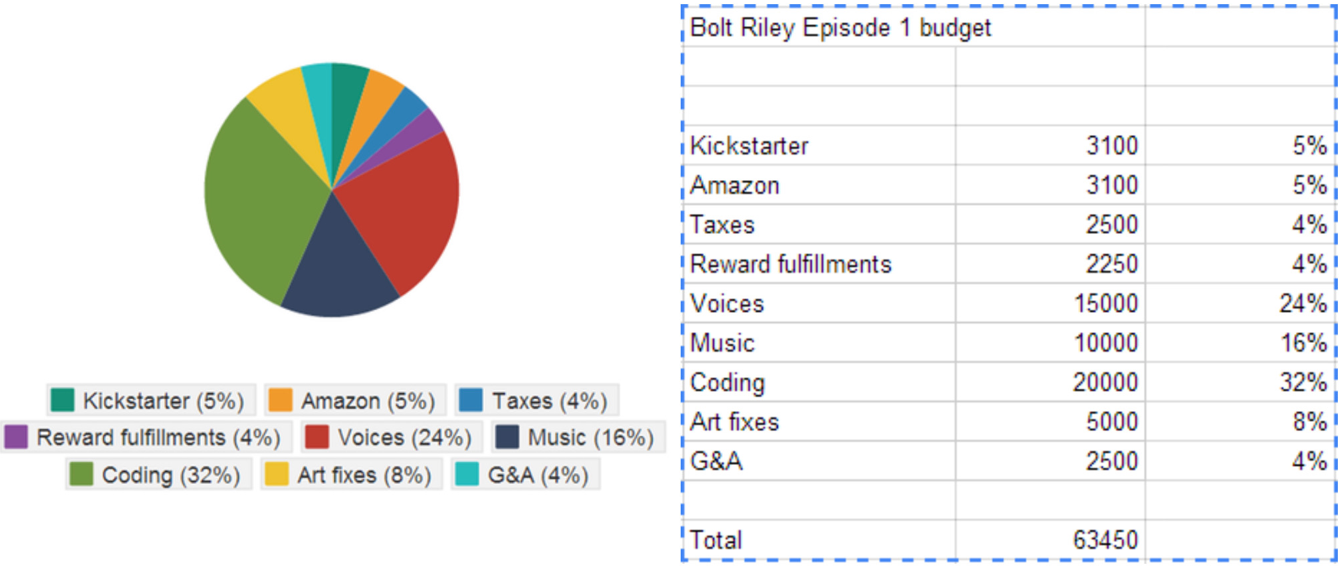
\includegraphics[keepaspectratio]{resources/images/image7.png}}

Quelle: Kickstarter.com, 2019

In einer Crowdfunding-Kampagne werden häufig Meilensteine eingerichtet,
nach deren Erreichen bestimmte Funktionen des Spieles implementiert
werden. Dies erhöht zum einen den Anreiz zur Investition für potentielle
Käufer, andererseits kann ein Spiel auch trotz nicht vollständigem
Erreichen einer Investitionssumme entwickelt werden. Weitere bekannte
Modelle der Finanzierung sind die Einnahme von Risikokapital durch
Investoren, welche im Gegenzug Unternehmensanteile erwerben (Perridon,
Steiner \& Rathgeber, 2016). Außerdem haben einige bekannte
Spieleentwickler durch Vorverkaufseinnahmen ihre Entwicklungen erst
ermöglichen können. Das Spiel wird bei Release dann häufig vorab an
diese Käufer vergeben, was für einige Fans des Produktes einen
eindeutigen Mehrwert zu bedeuten scheint.

\textbf{4.3.3 Vertriebs-, Finanzierungs- und Marketingmix}

Der Hersteller Game Workshop hat zusammen mit dem Entwicklungsstudio
Play Fusion für das Spiel ‚Warhammer Age of Sigmar: Champions` eine
geteilte Vermarktungsstrategie gewählt. Game Workshop verkauft zu ihrem
Free-to-Play Titel neben den üblichen In-App-Käufen, zusätzlich
gedruckte Sammelkarten, mit denen der Spieler neue Inhalte und
Erweiterungen freischalten kann. Diese Kartensets sollen Online zu
kaufen sein, in sogenannten Onlineshops. Die Warhammer-Reihe umfasst
viele verschiedene Arten von Spielen, analoge sowie digitale und besitzt
eine weltweite Fangemeinde. So konnten die Entwickler in zehn Tagen nach
Einführung eines der sogenannten ‚Booster Packs` fast zehn Millionen
Karten verkaufen (PRNewswire, 2018). Das dazu gehörige digitale
Handy-Spiel wird in den großen App-Stores, Google Play (Android Geräte)
und Apple Store (iPhones und iPads) angeboten. Das BenBox.org Spiel für
Tablet-Computer kann auf unterschiedliche Weise vertrieben, finanziert
und beworben werden. Diese sollen nun in Kürze beschrieben werden um
anschließend eine Entscheidung bezüglich der besten
Vermarktungsstrategie zu treffen.

Vertrieb:

\begin{itemize}
\tightlist
\item
  Festpreis-Vermarktung und Vertrieb durch Publisher oder App-Stores
\item
  Free-to-Play Vermarktung mit In-App-Käufen über App-Stores
\item
  Free-to-Play Vermarktung mit Werbung über App-Stores
\item
  Free-to-Play Vermarktung über App-Stores mit Käufen von Spielkarten
  über eine Onlinehandel-Plattform
\item
  Vertrieb an Schulen mittels Länderfinanzierung
\item
  Vertrieb in Kooperation mit einer GKV und gleichzeitiger Bezuschussung
\end{itemize}

Finanzierung:

\begin{itemize}
\tightlist
\item
  Eigenkapitalfinanzierung durch den Hersteller
\item
  Fremdkapitalfinanzierung durch Banken
\item
  Risikokapital durch Investoren
\item
  Vorverkaufs-Finanzierung durch Privatinvestoren
\item
  Crowdfunding-Finanzierung durch Privatinvestoren
\item
  Fördergelder durch z.B. den Bundeshaushalt
\end{itemize}

Marketing (nach Schön):

\begin{itemize}
\tightlist
\item
  Aussagekräftige Beschreibung des Produktes (Schlagwörter verwenden)
\item
  Erstellen und senden von Trailer und Werbevideo (innovative
  Spielinhalte)
\item
  Werbung in Foren (Entwickler-, Fan- und Spieleforen)
\item
  Bewertung der App durch Nutzer (Anfragen stellen an Testportale)
\item
  Werbung in sozialen Netzwerken (Facebook, Instagram, Twitter etc.)
\end{itemize}

(Schön, 2013)

\begin{itemize}
\tightlist
\item
  Werbung auf Webseite einer GKV
\end{itemize}

Wie in den zuvor beschriebenen Entwicklungen gezeigt, können diese
Strategien miteinander kombiniert werden, um so eine geteilte
Vertriebs-, Finanzierungs- und Marketingstrategie zu betreiben.

\textbf{4.4 Ökonomische Betrachtungen eines Corporate Games}

Nach dieser eingehenden Betrachtung der Finanzierung und Vermarktung von
Serious Games, soll in Kürze, im Hinblick auf eine Übertragung des
Spielansatzes auf eine erwachsene Zielgruppe, eine mögliche Strategie
für ein Corporate Game besprochen werden. Für eine erwachsene Zielgruppe
gelten andere Regeln, sowohl für Design und das UI eines Spieles, aber
insbesondere auch für dessen Vermarktung. Erwachsene Anwender können im
Gegensatz zu Kindern In-App-Käufe tätigen, da sie voll geschäftsfähig
sind. Bei einem Corporate Game kann also für ein Angebot mit diesem
Monetarisierungsansatz gearbeitet werden. Ob zusätzlich Werbung
geschaltet wird, sei zu prüfen. Darüber hinaus kann die Applikation
einen festen Preis haben, bzw. ein Abo-Modell nutzen. Zur
Monetarisierung kann zusätzlich der Präventionsleitfaden herangezogen
werden, um eine geldliche Entlastung für die Nutzer zu erwirken. Die
Primärprävention nach §20 SGB V bietet Anbietern von präventiven
Gesundheitskursen die Möglichkeit, sich zertifizieren zu lassen. Die
Zentrale Prüfstelle für Prävention (ZPP) organisiert dazu
versicherungsübergreifend die Präventionsangebote der GKVs. Unter der
Rubrik IKT (Informations- und Kommunikationstechnologie-basierte) sind
auch digitale Kurse einzureichen. Zu den für Anbieter zertifizierbaren
Kursen zählen ‚Blended Learning`, ‚Onlinekurse`, ‚Fernkurse`,
‚Gesundheitscoaching für Gruppen`, ‚Game based learning / Serious Games
/ e-Teaching` oder ‚Telefoncoaching`. Wird ein IKT Kurs von der ZPP nach
§20 Präventionsleitfaden zertifiziert, kann der Kursteilnehmer bei
erfolgreicher Teilnahme die Kosten anteilig, häufig 75 bis 150 € pro
Kurs, erstattet bekommen. Diese Förderung würde auch für minderjährige
Versicherte gelten, diese werden unter der Bezeichnung
Familienversicherte in den Mitgliederregistern der Gesetzlichen
Krankenkassen geführt. Die Erwachsene Zielgruppe wird oftmals durch die
Bewerbung der Kurse auf den Webseiten der Krankenkassen erreicht. Diese
übermitteln automatisiert, aus den Datenbeständen der ZPP, die Kursdaten
auf ihre eigenen Webportale. Außerdem kann ein Anbieter von digitalen
Präventionsangeboten jede Form der verteilten Print-, Online- und
Sozial-Media-Werbung schalten, sowie lokale Werbeflächen nutzen.

\section{5 Ergebnisse}\label{ergebnisse}

Von 22 Kindern der Klasse haben 15 an der Umfrage, deren Teilnahme
freiwillig war, teilgenommen. Das entspricht einer Teilnahmequote von
knapp 70 \%. Somit ist n = 15. Die Gruppe bestand aus acht Mädchen und
sieben Jungen. Der Altersschnitt lag bei Studiendurchführung bei 8,4
Jahren. Im ‚Item 1` (Abb. 5.1) wurde die Beliebtheit der Protagonisten
erfragt. Hier ist ersichtlich, dass die ‚BenBox` die höchste Beliebtheit
aufweist. Damit hat der Namensgeber des Spiels zu 100 \% der abgegebenen
Stimmen mit der besten Bewertung ‚Super` erhalten. An zweiter Stelle
befindet sich ‚SAM` mit elf Stimmen (73 \%), dicht gefolgt von ‚SEB` mit
zehn Stimmen (67 \%). Die Protagonistin ‚Emmi` bekam in der Kategorie
‚Ganz ok` mit sechs die häufigste Stimmenanzahl, was 40 \% der
abgegebenen Stimmen entspricht.

Abb. 5.1: Item 1

\pandocbounded{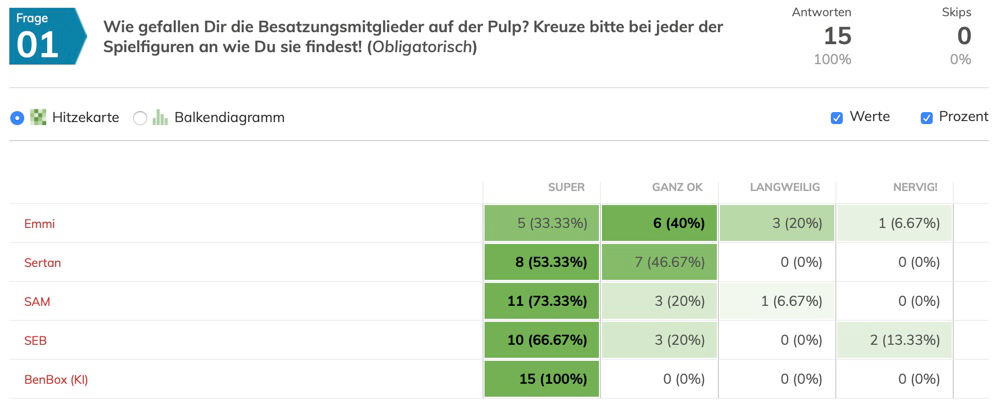
\includegraphics[keepaspectratio]{resources/images/image8.png}}

Quelle: Eigene Datenerhebung

Das ‚Item 2` (Abb. 5.2) zielte auf die Kaufgewohnheiten der Schüler ab.
Die Kinder sollten angeben, wofür sie ihr Taschengeld ausgeben. Sticker
und Sammelkarten wurde von neun Kindern angegeben, das waren 28 \% der
abgegebenen Stimmen. Da eine Mehrfachauswahl möglich war, entspricht
dies 60 \% der Kinder. Süßigkeiten und dergleichen, sowie digitale
Spiele wurden achtmal bzw. von 53 \% der Kinder ausgewählt.

Abb. 5.2: Item 2

\pandocbounded{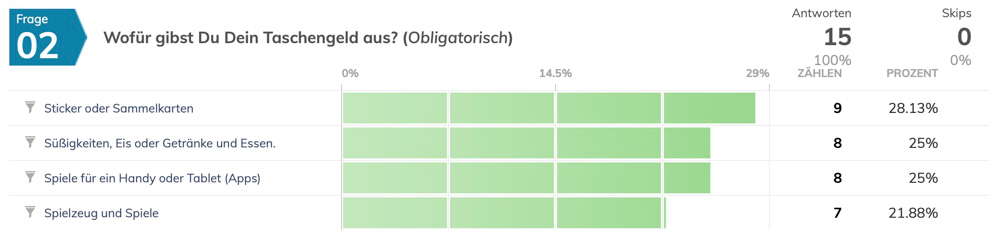
\includegraphics[keepaspectratio]{resources/images/image9.png}}

Quelle: Eigene Datenerhebung

Die Frage nach der Spielform in ‚Item 3` (Abb. 5.3) beantworteten zehn
Kinder mit der höchsten Wertung. Das entspricht ⅔ der Spieler. Weitere
vier Kinder fanden diese Art von Spiele ‚Ganz gut`, ein Kind selektierte
die Antwortkategorie ‚Blöd`.

Abb. 5.3: Item 3

\pandocbounded{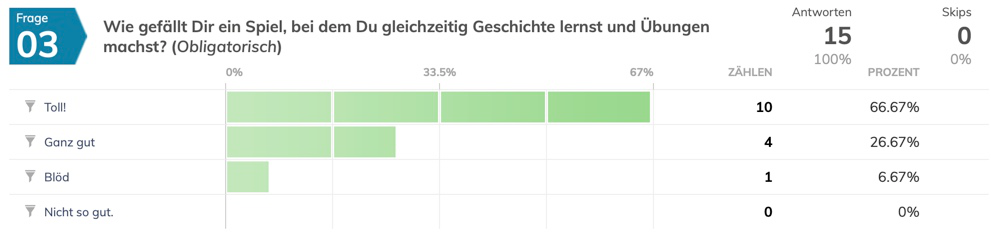
\includegraphics[keepaspectratio]{resources/images/image10.png}}

Quelle: Eigene Datenerhebung

Die Frage nach dem Spannungsgrat (‚Item 4`) der Geschichte (Abb. 5.4),
sowie dem Humor, zielte auf die erzählerische Darbietung ab. ‚Ja, ich
finde die Geschichte toll!{}` konnte mit 14 Stimmen 93 \% erreichen. Nur
eine Wertung mit der Kategorie ‚Die Geschichte ist nicht so gut`.

Abb. 5.4: Item 4

\pandocbounded{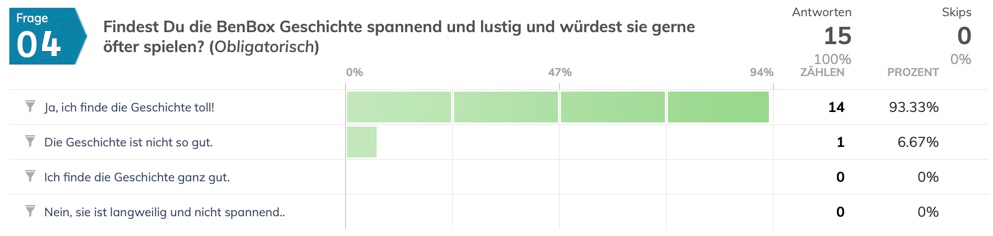
\includegraphics[keepaspectratio]{resources/images/image11.png}}

Quelle: Eigene Datenerhebung

Schlussendlich wurde in der Umfrage im ‚Item 5` (Abb. 5.5) erfragt, ob
das Kind bereit wäre Taschengeld für das Spiel auszugeben und wenn ja
wieviel. Die höchste Häufigkeit hatte die Kategorie ‚10 Euro` mit acht
abgegebenen Stimmen. Fünf Kinder stimmten für ‚5 Euro` ab. Im
arithmetischen Mittel bedeutet das einen Wert von 7 €.

Abb. 5.5: Item 5

\pandocbounded{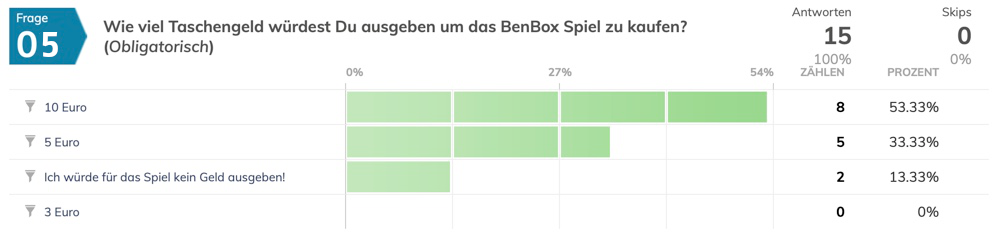
\includegraphics[keepaspectratio]{resources/images/image12.png}}

Quelle: Eigene Datenerhebung

Im Durchschnitt wurden von den Kindern am Ende des Spieles beim finalen
Punktestand 2,1 Karten abgegeben. Im Weiteren wurde erhoben, wie die
Paarungen die Spielkarten eintauschten. Daraus ergab sich folgender
Datensatz:

Paarung (Prg) 1: 3 und 3 Karten; Prg 2: 1 und 1 Karten; Prg 3: 2 und 1
Karten; Prg 4: 3 und 3 Karten; Prg 5: 0 und 0 Karten; Prg 6: 3 und 3
Karten; Prg 7: 3 und 3 Karten; Prg 8: 3 Karten (zweiter Spieler ohne
Wertung da eine Betreuerperson).

Somit trafen sechs von sieben Paarungen die gleiche Entscheidung
bezüglich der Ausgabe der Spielkarten. Das entspricht einer Häufigkeit
von 86 \% identischer Endscheidung.

\section{6 Diskussion}\label{diskussion}

Die BenBox.org Unternehmung muss einen ökonomischen Nutzen ausweisen,
sprich ein effizientes Vertriebssystem beinhalten,
Finanzierungssicherheit vorweisen, um die Entwicklungskosten zu tragen,
sowie ein zielgruppenorientiertes Marketing aufweisen. Mit einem
Monetarisierungskonzept in dem mittels In-App-Käufe Geld eingenommen
wird, kann bei Kindern aus zwei Gründen nicht gearbeitet werden. Erstens
verfügt die Zielgruppe durch ihre eingeschränkte Geschäftsfähigkeit
nicht über einen entsprechenden zahlungsfähigen Zugang zu den
Vertriebskanälen App-Stores (Google und Apple), zweitens kann diese
Zielgruppe aus pädagogischen und medizinischen Gründen nicht über die
eigenen Gesundheitsausgaben entscheiden.

In der Altersgruppe ist indes eine erhöhte gruppendynamische Komponente
zu identifizieren, was auch die Ergebnisse der fast immer gleichen
Spielkartenabgaben am Spielende nahelegt. Dieser Aspekt kindertypischen
Verhaltens soll im vorgestellten Produkt in keiner Weise die zu
treffenden Entscheidungen über Gesundheitsvorsorge beeinflussen. An
dieser Stelle kann von mindestens zwei unterschiedlichen Betrachtungen
ausgegangen werden. Zum einen ist ein starker Gemeinschaftssinn positiv
für die sozialen Fähigkeiten eines Kindes, eine Gruppenzwangsituation
zum anderen eher als hinderlich im Individualisierungsprozess des Kindes
zu verstehen. Wenngleich die Antworten der Kinder in der Studie
grundsätzlich als ehrlich, also ohne Hintergedanken oder Umfrage
steuernde Absichten gemacht wurden, kann ein Kind in dieser Altersgruppe
sicherlich nicht als allein verantwortlich bezüglich der eigenen
Gesundheit und Entwicklung gelten. Somit muss das BenBox.org Marketing
einen Fokus auf den Wert der Gesundheit legen und die Reduzierung von
Gesundheitskosten versprechen. Dieses Argument soll zu allererst an die
Krankenkassen adressiert werden.

Einen zweiten Fokus wird auf die Entwicklung und Ausbildung des Kindes
gerichtet sein. Dass die digitalen Medien nicht mehr aus dem Leben von
Kindern wegzudenken sind, ist ein nicht zu bestreitender Fakt.
Vielfältiger individueller Nutzen, Unterhaltung, kommunikatorische
Vernetzung und die Verknüpfung vormals verteilter Daten sind der Nutzen
den ein Kind daraus ziehen kann. Lag die Verantwortung über die
Unterstützung des Kindes in seinem Aufwachsen zuvor fast ausschließlich
bei den Eltern und Lehrern, kann diese nun aufgeteilt werden. Dies
können auch digitale Anwendungen leisten, allerdings nur sofern die
Sicherheit der Angebote garantiert ist.

Als dritter Fokus, gilt es die eigentliche Zielgruppe Kinder, durch ein
spannendes und herausforderndes Spiel, zu erreichen. Aus den
Umfrageergebnissen geht hervor, dass das Prototyp-Produkt eine für
Kinder angemessene Bild- und Textsprache verwendet hat. Außerdem konnten
die eingesetzten Protagonisten die Zielgruppe ansprechen, sowie zum
Projizieren (Erwartungen) und Identifizieren (Selbstreflexion) anregen.
Das belegen die Umfrage ‚Items 1` und ‚Item 4` in der Studie. Einzig und
allein die Protagonistin ‚Emmi` mit durchschnittlichen Bewertungen, muss
überdacht und evtl. neu konzipiert werden. Notwendigerweise braucht die
Geschichte eine vernünftige bzw. erwachsene Person, was zu einer solchen
Bewertung durch Kinder führen kann. Da einige Grafiken des Spieles
teilweise in frühen Entwurfszuständen implementiert wurden, um Fristen
einzuhalten und die Kosten für den Prototypen zu senken, kann für ein
produktionsreifes Produkt auch insgesamt von einer höheren Qualität
ausgegangen werden. Ein Serious Game für Gesundheit ist bei Kindern,
einer Zielgruppe, die grundsätzlich lernfreudig ist, ‚Item 3` der
Umfrage kann diese Forschungshypothese bestätigen, ein wachendes
Spielegenre und verspricht Marktanteile. In der Umfrage gaben die Kinder
an, im Schnitt 7 € ihres Taschengeldes investieren zu wollen. Diese Zahl
spricht für die Eigenmotivation der Zielgruppe dieses Angebot zu nutzen.
Allerdings kann ein durchschnittlicher App-Preis von ca. 4 € für die
BenBox.org nicht angesetzt werden. Auch der durchschnittliche Preis für
Vollpreis-Titel von ca. 40 € soll nicht veranschlagt werden. Die
Mehrwerte, Hinzuwachs des gesundheitlichen und kulturellen Kapitals,
müssen den Entscheidern (Krankenkassen und Eltern) beim Kontakt mit dem
Produkt allgegenwärtig sein. Das Ziel der Unternehmung ist es somit,
einen Kauf des BenBox.org Spieles seitens der Eltern zu generieren, die
dieses Angebot über die Webseite der Krankenkasse offeriert bekommen,
niemals jedoch dem Kind alleine eine Kaufentscheidung zuzubilligen.

Als Kalkulationsgrundlage für die Preisgestaltung des Angebotes dient
die angestrebte Kooperation mit der TK und die Bewerbung der BenBox.org
über die ‚\href{http://www.tk.de}{www.tk.de}` Webseite. Von den 2,5
Millionen Familienversicherten sind schätzungsweise 20 \% also 500.000
der Altersgruppe 6 bis 13 Jahre zuzuordnen. Daraus ergibt sich bei einer
anvisierten Marktdurchdringung von 5 \% eine zu erwartende
Zielgruppengröße von ca. 25.000 Nutzern. Im Hinblick auf die reinen
Entwicklungskosten, es wird eine Summe von 150.000 € kalkuliert,
bedeutet dies Umlagekosten von 6 € pro Nutzer. Dazu kommen
Marketingkosten und diverse weitere Aufwendungen wie die Unterhaltung
einer Geschäftsstelle von insgesamt 50.000 €. So kann von einer Umlage
von zusätzlichen 2 € pro verkauften Artikel gerechnet werden. Die
Produktionskosten setzen sich aus den Kostenstellen der Tabelle 6.1
zusammen:

Abb. 6.1: Tabelle - Produktionskosten

\pandocbounded{\includegraphics[keepaspectratio]{resources/images/image13.x-emf}}

Quelle: eigene Darstellung

Die Grenzkosten des Produktes sind sehr gering, da bei einem digitalen
Produkt keine weiteren Materialien zum Einsatz kommen müssen und nur der
Vertriebsweg (anteilige Umsatzausschüttung) und Geschäftsbetrieb Kosten
verursachen. Daraus ergibt sich eine maximale Skalierbarkeit des
Produktes von Seiten der Produktion. Eine Kooperation mit einer Privaten
Krankenkasse (PKV) kann somit eine gute Perspektive sein, um weitere
Nutzer zu gewinnen. Diese Zusammenarbeit sollte keine Probleme seitens
der bestehenden Partnerschaft mit der TK mit sich bringen, da zwischen
den beiden Krankenkassen keine direkte Mitbewerberschaft besteht. Die
gesamten Produktionskosten (Tab. 6.2) von 200.000 € sollen mittels
dieser Kapitalquellen erschlossen werden:

Abb. 6.2: Tabelle - Kapitalquellen

\pandocbounded{\includegraphics[keepaspectratio]{resources/images/image14.x-emf}}

Quelle: eigene Darstellung

Fiele eine dieser Kapitalquellen aus, soll zuerst mittels Förderungen am
Finanzplan festgehalten werden, bevor Kosteneinsparungen diskutiert
werden.

Durch die Kooperation mit der Krankenkasse soll eine Zielgruppe von
mindestens 25.000 potentiellen Versicherten, Kinder im Alter von 6 bis
13 Jahren, erreicht werden. Die Vertriebsstrategie soll zweiteilig sein:

\begin{itemize}
\tightlist
\item
  Zum einen kann das Spiel über die Mitgliedschaft der Gesetzlichen
  Versicherung subventioniert erworben werden, es ist dementsprechend
  kein Free-to-Play Titel. Der Kaufpreis soll mit 99 € angesetzt werden,
  was das empfohlene Taschengeldniveau eines Kindes im Alter von 6 bis
  13 deutlich übersteigt (Nissen, o. J.). Die jeweilige Krankenkasse
  bezuschusst allerdings bei regelmäßiger Teilnahme abschließend den
  Präventions-Kurs mit 75 € und dem Käufer entsteht somit nur eine
  geringe finanzielle Belastung. Es ist anzunehmen, dass eine
  Rückenschule, welche als Serious Game digital, also vernetzt zu nutzen
  ist, gegenüber den Sportangeboten in dieser Altersklasse einen
  besseren Stand hat, als eine reguläre lokal und terminiert
  stattfindende Kinderrückenschule. Deren Verbreitungs- und damit
  Bekanntheitsgrad ist grundsätzlich deutlich unter denen der
  Rückenschulen für Erwachsene anzunehmen. Letztendlich müssen die
  Entscheider, die Eltern, überzeugt werden, um diesen im Vergleich zum
  klassischen Spielemarkt deutlich höheren Verkaufspreis erzielen zu
  können. Der Hinweis, dass es sich um eine Gesundheitsdienstleistung
  handelt, muss also zwingend erbracht werden. Durch die Verknüpfung von
  Spiel und Gesundheitsprophylaxe, soll eine entsprechende maximale
  Nutzungszeit, orientiert an der typischen Kursdauer eines
  Offline-Kursangebotes, eingerichtet werden. Dies ist auch im Hinblick
  auf die Medienkompetenz der Kinder anzustreben.
\item
  Der Zweite Vertriebsansatz soll die Möglichkeit sein, Erweiterungen
  anzubieten. Die Erweiterungen des BenBox.org Spieles, in Form von
  neuen Übungen und Inhalten, geschieht nicht durch klassische
  In-App-Käufe, sondern durch den Erwerb von Spielkarten. Diese
  Spielkarten sind über einen Online-Shop zu erwerben und mit
  handelsüblichen Bezahlmethoden wie Überweisung, Rechnung, PayPal und
  dergleichen zu bezahlen. Mit den Spielkarten kann das Kind
  anschließend auch außerhalb der digitalen Spielumgebung spielen, sowie
  Zusatzinhalte im Serious Game freischalten. Hier ist von einer
  Hybridisierung zu sprechen, wie sie einige Spieleanbieter zuvor
  betrieben haben.
\end{itemize}

Der Kauf wird nur volljährigen Personen angeboten, also Personen deren
Medienkompetenz und Mündigkeit als ausreichend ausgebildet anzunehmen
ist. Die BenBox.org verfolgt demnach eine Monetarisierungsstrategie, bei
der die Bezahlmechanismen von den Eltern bzw. den Erziehungsberechtigten
ausgelöst werden müssen. Dementsprechend muss sich das Marketing auf die
Eltern konzentrieren. Um das Produkt jedoch bei einer der Gesetzlichen
Krankenkassen platzieren zu können, muss der Mehrwert der entsprechenden
Versicherung schlüssig dargestellt werden. Hier ist das entscheidende
Mittel, auf die Kosten von Gesundheit eines Kindes hinzuweisen. Es ist
nicht anzuraten, profitorientierten Unternehmen wie Apple, Google und
vergleichbare im Schutz von Minderjährigen voll zu vertrauen, unabhängig
davon, wie umfangreich diese Technologieanbieter die Schutzfunktionen in
ihren Produkten implementiert haben und diese bewerben.

Dass ein solches Angebot innerhalb des üblichen Vermarktungsweges über
einen App-Store erfolgreich vertrieben werden kann, ist zu bezweifeln.
Zum einen verlangen der ‚Google Play-Store` und ‚Apple App-Store` hohe
Umsatzbeteiligungen, was zu einer Schmälerung des Gewinnes führen würde,
zum anderen, ist der Verkaufspreis ungleich höher als der der
Konkurrenzprodukte. Allenfalls können die App-Stores der Bereitstellung
des Produktes (Download) dienen, jedoch nicht der Monetarisierung über
die dort gängige Bezahlinfrastruktur.

\section{7 Fazit und Ausblick}\label{fazit-und-ausblick}

Ob das beschriebene Serious Game ohne eHealth-Kooperationspartner (GKV)
in den App-Stores gegen das große Angebot an Spiele-Apps mit In-App-Kauf
Funktion und Werbung bestehen kann, bleibt zu klären. Apps ohne
In-App-Kauf Funktion generieren den App-Store-Anbietern keine Umsätze,
genauso wie jene die auf Werbeeinblendungen verzichten. Dies könnte sich
negativ auf das Ranking im jeweiligen App-Store auswirken.

Über den Vertriebsweg des Kartenverkaufes, ist ebenso denkbar eine
Private Krankenkasse, die üblicherweise keine Subventionierungen zu
Präventionsdienstleistungen ausschüttet, als Kooperationspartner zu
gewinnen. In diesem Fall muss der Verkaufspreis von 99 € gesenkt werden,
um eine breite Nutzergruppe anzusprechen. Dahingehend, dass eine klar
umschriebene Zielgruppe definiert wurde, sollte diese PKV sinnvoller
Weise eine passende Mitgliederstruktur ausweisen. Der bisher als
Prototyp entwickelte eHealth Ansatz soll dazu weiterentwickelt werden.
Schlussendlich soll die BenBox.org eine PI werden und dem Nutzer
aufzeigen, wie er sich am besten bzw. am schnellsten weiterentwickeln
kann. Dieses Assistenz-System soll allerdings nie autonome
Entscheidungen für die Kinder treffen, sondern allenfalls den
Stellenwert einer Entscheidungshilfe innehaben. Weiterhin werden neue
Programmfunktionen benötigt, um die Spiel- und Lerninhalte besser und
variantenreicher vermitteln zu können. Diese Erweiterungen können nur
durch den Zukauf von externen Programmierern realisiert werden bzw. der
Rekrutierung von Mitarbeitern mit entsprechenden Fähigkeiten. Da
Darmstadt eine hoch angesehene Hochschule im Informatiksektor
aufzuweisen hat, kann der Bedarf an Fachkräften dort gestillt. Als
kostengünstige Alternative könnten Programmierer aus dem Projekt der
Digital School of Integration (kurz: ReDi), welche in München und Berlin
Schulen betreibt, könnten für diese Zwecke akquiriert werden. ReDi
schult Flüchtlinge aus Krisengebieten im Programmieren. Die Entwicklung
der BenBox.org soll Cross-Plattform erfolgen. Das heißt, es sollen
verschiedene Versionen für die beiden wichtigen mobilen Betriebssysteme,
Android und iOS, entwickelt werden. Dieser Schritt kann kosteneffizient
mit der Game-Engine Unity erfolgen (Thomas, 2018). Stadia kann ein
zusätzlicher Vertriebskanal sein, der einen erweiterten großen
Absatzmarkt von Gelegenheitsspielern erschließt und aufgrund des
Abo-Systems eine stetige Einnahmequelle bedeuteten würde. Es steht
außerdem in Planung, die neue Darstellungsform der Virtual Reality zu
implementieren. Dazu würde die BenBox.org als BenBox.VR in Zukunft
neuaufgelegt werden. Die BenBox.VR würde dann die Zielgruppe Erwachsene
erschließen, als ein Corporate Game. In Kooperation mit der Hochschule
Darmstadt und Prof. Philipp Thesen, der im Studiengang Industriedesign
im Fachbereich Gestaltung die Mensch-System-Interaktion erforscht, soll
ab Oktober 2019 dazu in Zusammenarbeit ein Prototyp der BenBox.VR
entstehen. Mit diesen technischen Voraussetzungen könnte eine PI
motorisch sinnvolle Bewegungen auf die VR-Brille projizieren, damit der
Nutzer neue Bewegungsstrategien und komplexe Koordinationsleistungen
ausprobieren und einstudieren kann. Durch die Erweiterung der
Produktpalette mit dem BenBox.VR Corporate Game, wäre eine
Diversifizierung erreicht und gleichzeitig verschiedene Absatzmärkte
anvisiert.

Das BenBox.org Spiel soll zum Teil durch Risikokapitalgeber, also mit
Geld von Investoren, finanziert werden. Um diese zu überzeugen, Kapital
in das Projekt zu investieren, soll ein sogenanntes Pitch Deck erstellt
werden, mit dem an speziellen Investoren-Veranstaltungen für das Produkt
geworben werden soll. Die Vorstellung des BenBox.org Prototypen erlaubt
die visuelle Präsentation des zukünftigen Produktes, was eine mögliche
Akquirierung von Investoren grundsätzlich erleichtert würde. Dazu würde
im Anschluss an diese Arbeit ein Businessplan erstellt, welcher einen
fundierten Finanzplan enthalten würde. Die Firma neuland.digital GmbH,
geführt von dem in Köln ansässigen Unternehmer Karl-Heinz Land, berät
Unternehmen in der digitalen Transformation und unterstützt Start-Ups
mit ihrem Netzwerk an Investoren. Neuland.digital GmbH soll für die
beiden Projekte Risikokapital einsammeln und darüber hinaus in der Rolle
des Publisher fungieren, um die termingerechte Produktion zu managen. Im
Anschluss an die Finanzierungsphase soll mit der Mitarbeitersuche
begonnen werden, um ein Team an tatkräftigen und innovativen Fachkräften
für die Umsetzung der BenBox.org und BenBox.VR zu akquirieren. Das für
diese Zwecke gegründete Unternehmen soll ‚Serious Ben Entertainment`
heißen und langfristig den zuvor beschriebenen ökonomischen Nutzen
erbringen. Das Unternehmen soll als GmbH geführt werden. Durch die gute
Reputation dieser Unternehmensform soll das noch fehlende Kapital von
einer Bank eingezogen werden. Außerdem soll parallel geprüft werden, ob
eine Förderung in Anspruch genommen werden kann. Fördermittel, zum
Beispiel die Games-Förderung der Bundesregierung, können helfen die
Finanzierbarkeit dieser zusätzlichen Funktionen zu gewährleisten. Eine
zusätzliche Kapitalquelle soll durch eine Crowdfunding-Kampagne
erschlossen werden. Es hat sich gerade im Computer-Spiele-Markt gezeigt,
dass sich hier große Mengen an Fremdkapital durch Privatinvestoren
erschließen lassen und durch die Verwendung von Meilensteinen die
Wahrscheinlichkeit einer Produktion erhöhen lässt. Die
Privatunterstützer sollen als Ausgleich dafür Merchandise Artikel und
andere Honorierungen bekommen, die je nach Höhe der finanziellen
Unterstützung ausgeschüttet würden.

Um im Vorfeld die Bekanntheit des innovativen Projektes zu steigern,
sowie um am starken Digital-Health-Cluster Netzwerk in der Region
Köln-Bonn zu partizipieren, soll die BenBox.org im Rahmen des Health-i
Award 2019 in der Kategorie ‚Junge Talente` am Wettbewerb mit
Einsendeschluss am 12. Juni diesen Jahres teilnehmen.

\section{Literaturverzeichnis}\label{literaturverzeichnis}

Adler, Dr. M., Ganzenberg, E., Martin, M., González, R., R. \& Schubert,
N. (2017). Media Activity Guide 2017: Mediennutzung im Blick.
Unterföhring: SevenOne Media GmbH.

Bathge, P. (2019).* Star Citizen: Crowdfunding-Summe überschreitet 222
Millionen US-Dollar*. Zugriff am 14.05.2019 unter:
https://www.gamestar.de/artikel/star-citizen-222-millionen-dollar-finanzierung,3342603.html

Baur, N. \& Blasius J. (2014). Handbuch Methoden der empirischen
Sozialforschung. Wiesbaden: Springer VS.

Becker, L. (2019). \emph{Apples WWDC 2019: iOS 13 mit Dunkelmodus,
Datenschutz und optimierter Leistung}. Zugriff am 8.6.2019 unter:
https://www.heise.de/mac-and-i/meldung/Apples-WWDC-2019-iOS-13-mit-Dunkelmodus-Datenschutz-und-optimierter-Leistung-4438243.html?hg=1\&hgi=39\&hgf=false

Beineke, J. (2019). \emph{Mobile Games: 24 Lieblingsspiele der
Heise-Redaktion für Smartphone. Spiele für Smartphones sind billige
Werbeschleudern, voll mit Mikrotransaktionen? Das muss nicht sein, wie
die liebsten Games der Heise Redakteure beweisen.} Zugriff am 6.6.2019
unter:
https://www.heise.de/ratgeber/Mobile-Games-24-Lieblingsspiele-der-Heise-Redaktionen-fuers-Smartphone-4431033.html?seite=all

Bensch, M. \& Raab-Steiner, E. (2012). Der Fragebogen (3. Aufl.). Wien:
Facultas Verlag- und Buchhandels AG.

Bourdieu, P. (1983). Ökonomisches Kapital, kulturelles Kapital, soziales
Kapital. In R. Kreckel (Hrsg.), \emph{Soziale Ungleichheiten}, S.
183-199. Göttingen: Schwartz.

Bucher, A. (2014). \emph{Psychologie der Spiritualität} (2. Aufl.).
Basel: Beltz Verlag.

Bundesjugendministerium (Hrsg.) (2017). \emph{Medienkompetenz stärken}.
Zugriff am 10.05.2019 unter
https://www.bmfsfj.de/bmfsfj/themen/kinder-und-jugend/medienkompetenz/medienkompetenz-staerken/75350

Bundesministerium für Bildung und Forschung (Hrsg.) (o. J.).
Digitalisierung in Bildung und Forschung. Zugriff am 9.6.2019 unter:
https://www.bmbf.de/de/open-access-das-urheberrecht-muss-der-wissenschaft-dienen-846.html

Daun., A. (2012). \emph{Starke Kinder -- Wollen wir die wirklich haben?
}Aachen: Karin Fischer Verlag GmbH.

Egger, L. (2009). \emph{The impact of Harry Potter on readers of his
age}. München: GRIN Verlag.

Euro-Informationen (Hrsg.) (2019). \emph{Die größten Krankenkassen:
Versicherte 2019}. Zugriff am 3.6.2019 unter:
https://www.krankenkassen.de/krankenkassen-vergleich/statistik/versicherte/aktuell/

Flothow, A., Kempf, H. D., Kuhnt, U. \& Lehmann, G. (Hrsg.) (2011).
\emph{KddR-Manual. Neue Rückenschule Professionelle Kurskonzeption in
Theorie und Praxis}. München: Elsevier GmbH.

Förstl, H. (2012). \emph{Theory of Mind. Neurobiologie und Psychologie
sozialen Verhaltens} (2. Aufl.). Heidelberg: Springer.

Gaschler, K. (2019). Optimierung in rasantem Tempo. \emph{Gehirn \&
Geist}, 5\_2019, 82-83.

game - Verband der deutschen Games-Branche (Hrsg.) (2018).
\emph{DEUTSCHER}

\emph{GAMES-FONDS. Modell für eine Games-Förderung des Bundes. }Zugriff
am 15.05.2019 unter:
https://www.game.de/wp-content/uploads/2018/04/2018-09-28-Deutscher-Games-Fonds.pdf

game - Verband der deutschen Games-Branche (Hrsg.) (2017). \emph{Gamer
kaufen häufiger Zusatzinhalte für Free-to-Play-Spiele und Co.} Zugriff
am 13.05.2019 unter
\url{https://www.game.de/gamer-kaufen-haeufiger-zusatzinhalte-fuer-free-to-play-spiele-und-co/}

Goldin, I. \& Kutarna, C. (2016). \emph{Die zweite Renaissance: Warum
die Menschheit vor dem Wendepunkt steht}. München: FinanzBuch Verlag.

Greiner, W., Schulenburg, J.-M. G., Vauth, C. (Hrsg.) (2008).
\emph{Gesundheitsbetriebslehre}. Bern: Verlag Hans Huber.

Gugutzer, R. \& Staack, M. (Hrsg.) (2015). \emph{Körper und Ritual.
Sozial- und kulturwissenschaftliche Zugänge und Analysen}. Wiesbaden:
Springer Fachmedien.

Günther, B. (2014). \emph{Apple erhält 30\% der Einnahmen von Microsoft
Office für iPad}. Zugriff am 22.05.2019 unter:
https://www.mactechnews.de/news/article/Apple-erhaelt-30-der-Einnahmen-von-Microsoft-Office-fuer-iPad-158076.html

Häckl, D. (2010). \emph{Neue Technologien im Gesundheitswesen.
Rahmenbedingungen und Akteure}. Wiesbaden: Gabler Verlag.

Heim, D. (2018). \emph{Supercell erklärt automatisierte Monetarisierung
in Clash Royale}. Zugriff am 10.05.2019 unter
https://www.newsslash.com/n/12669-supercell-erklaert-automatisierte-monetarisierung-in-clash-royale

Hennings, S. (2012). Patientenbefragung als Chance für
Qualitätsmanagement und Praxismarketing. Hamburg: Diplomica Verlag GmbH.

Herbig, D. (2019). \emph{Google Stadia: Cloud-Gaming-Dienst kostet 10
Euro im Abo}. Zugriff am 7.6.2019 unter:
https://www.heise.de/newsticker/meldung/Google-Stadia-Cloud-Gaming-Dienst-kostet-10-Euro-im-Abo-4441177.html

Hollenberg, S. (2016). \emph{Fragebögen. Fundierte Konstruktion,
sachgerechte Anwendung und aussagekräftige Auswertung}. Wiesbaden:
Springer Fachmedien.

Holler, A. (2012). Freundschaft ist Wichtig. Was Kinder meinen aus
SpongeBob Schwammkopf gelernt zu haben. \emph{TELEVIZION, 25/2012/2},
19-22.

Informatik und Gesellschaft (2009). \emph{Schwache KI und Starke KI. }
Zugriff am 29.03.2019 unter
http://www.informatik.uni-oldenburg.de/\textasciitilde iug08/ki/Grundlagen\_Starke\_KI\_vs.\_Schwache\_KI.html

IZI (Internationales Zentralinstitut für das Jugend- und
Bildungsfernsehen) (Hrsg.) (2019). \emph{Grunddaten Kinder und Medien
2019}. Zugriff am 04.03.2019 unter:
https://www.br-online.de/jugend/izi/deutsch/Grunddaten\_Kinder\_u\_Medien.pdf

Jæger, M. M., Karlson, K. (2018). Cuiltural capital and educational
inequality. A counterfactual analysis. \emph{Sociological Science 5},
DOI: 10.15195/v5.a33, 775-795.

Kallus, K. W. (2016). \emph{Erstellung von Fragebogen }(2. Aufl.). Ulm:
CPI-Ebner \& Spiegel.

Kelava, A. \& Moosbrugger, H. (2012). \emph{Testtheorie und
Fragebogenkonstruktion }(2. Aufl.). Heidelberg: Springer.

Krämer, S. (2019). Die Kulturtechnik der Verflachung. Zugriff am
7.6.2019 unter: https://19.re-publica.com/de/news/rp19-sybille-kraemer

Kroeber-Riel, W. \& Esch, F. (2015). \emph{Strategie und Technik der
Werbung. Verhaltens- und neurowissenschaftliche Erkenntnisse} (8.
Aufl.). Stuttgart: W. Kohlhammer GmbH.

Lammenett, E. (2014). \emph{Praxiswissen Online-Marketing. Affiliate-
und E-Mail-Marketing, Suchmaschinenmarketing, Online-Werbung, Social
Media, Online-PR} (4. Aufl.). Wiesbaden: Springer Fachmedien.

Land, K.-H. (2018). \emph{Erde 5.0. Die Zukunft provozieren}. Köln:
FutureVisionPress e.K..

Legner, A. (1989). \emph{Reliquien. Verehrung und Verklärung}. Köln:
Greven \& Bechtold GmbH.

Lay, R. (1995). \emph{Nachkirchliches Christentum. Der lebende Jesus und
die sterbende Kirche} (2. Aufl.). Ulm: Ebner.

Leven, D. \& Knaak, P. (2017). Viel zu verlieren. \emph{Stiftung
Warentest, 7/2017}, 26-31.

Martin-Niedecken, A. L. \& Mekler, E. D. (2018). The ExerCube:
Participatory Design of an Immersive Fitness Game Environment. In S.
Göbel, A. Garcia-Agundez, T. Tregel, M. Ma, J. Baalsrud Hauge, M.
Oliveira, T. Marsh, P. Caserman (Hrsg.), \emph{Serious Games - 4th Joint
International Conference, JCSG 2018 }(S. 263-275). Cham: Springer Nature
Switzerland AG.

Mummendey, H. D. \& Grau, I. (2014). \emph{Die Fragebogenmethode.
Grundlagen und Anwendung in Persönlichkeits-, Einstellungs- und
Selbstkonzeptforschung} (6. Aufl.). Göttingen: Hogrefe.

Niebert, F. (2018). \emph{HYBRID-BRETTSPIELE: DIE NEUE GENERATION DES
SPIELENS}

\emph{Das mobile Endgerät nimmt eine wichtige Rolle ein}. Zugriff am
24.05.2019 unter:
https://www.trendyone.de/news/hybrid-brettspiele-die-neue-generation-des-spielens

Nissen, T. (o. J.). \emph{Taschengeldtabelle. Wie hoch sollte das
Taschengeld sein? Regeln, Ratgeber zum Ausdrucken und Expertenmeinung}.
Zugriff am 31.05.2019 unter:
https://www.arbeitsgemeinschaft-finanzen.de/soziales/taschengeld/

Nvidia (Hrsg.) (o. J.). \emph{Deep Learning}. Zugriff am 3.6.2019 unter:
https://developer.nvidia.com/deep-learning

O'Neilla, H. M., Maarbjerg, S. J., Crane, J. D., Jeppesen, J.,
Jørgensen, S. B., Schertzer, J. D., Shyroka, O., Kiens, B., van
Denderen, B. J., Tarnopolsky, M. A., Kemp, B. E., Richter E. A. \&
Steinberg, G. R. (2011). \emph{AMP-activated protein kinase (AMPK) β1β2
muscle null mice reveal an essential role for AMPK in maintaining}

\emph{mitochondrial content and glucose uptake during exercise}. Zugriff
am 3.6.2019 unter: https://www.pnas.org/content/108/38/16092

Perridon, L., Steiner, M. \& Rathgeber, A. (2016).
\emph{Finanzwirtschaft der Unternehmung }(17. Aufl.). München: Verlag
Franz Vahlen.

Porst, R. (2014). \emph{Fragebogen. Ein Arbeitsbuch}. Wiesbaden:
Springer VS.

PRNewswire (Hrsg.) (2018). \emph{PlayFusion: Sammelkarten-Booster Packs
für ``Warhammer Age of Sigmar: Champions'' ausverkauft}. Zugriff am
15.05.2019 unter: \url{https://www.presseportal.de/pm/130009/4036737}

Pyka, P. (2017). \emph{MARKETING 4.0. Der Leitfaden für das Marketing
der Zukunft}. Frankfurt: Campus Verlag.

Russell, S. J. \& Novig, P. (2016). \emph{Artificial Intelligience: A
modern approach} (3. Aufl.). Boston: Pearson.

Schellhammer, S. (2002). \emph{Bewegungslehre. Motorisches Lernen aus
Sicht der Physiotherapie}. Landshut: Urban \& Fischer Verlag.

Schmitt, F., Christopher, S. M., Tumanov, K., Weiss, G. \& Möckel, R.
(2018). Evaluating the Adoption of the Physical Board Game Ludo for
Automated Assessments of Cognitive Abilities. In S. Göbel, A.
Garcia-Agundez, T. Tregel, M. Ma, J. Baalsrud Hauge, M. Oliveira, T.
Marsh, P. Caserman (Hrsg.), \emph{Serious Games - 4th Joint
International Conference, JCSG 2018 }(S. 263-275). Cham: Springer Nature
Switzerland AG.

Schmitt-Sausen, Nora (2018). \emph{Deutsches Ärzteblatt 2018. USA: Das
Digitalzeitalter entfaltet sein Potential}. Deutsches Ärzteblatt 2018,
115 (15): A-698 / B-600 / C-601.

Schneider, F. (2017). Entwickler verrät: Werbung bringt deutlich mehr
als In-App-Kauf zur Deaktivierung von Werbung. Zugriff am 22.05.2019
unter:
https://www.appgefahren.de/entwickler-verraet-werbung-bringt-deutlich-mehr-als-in-app-kauf-zur-deaktivierung-von-werbung-191605.html

Scholl, A. (2018). \emph{Die Befragung }(4. Aufl.). UVK
Verlagsgesellschaft mbH.

Schön, D. (2013). \emph{Android-App bewerben: Die 5 besten
Marketing-Tipps.} Zugriff am 15.05.2019 unter:
https://praxistipps.chip.de/android-app-bewerben-die-5-besten-marketing-tipps\_20262

Sinclair, J., Hingston, P., \& Masek, M. (2009). Exergame development
using the dual flow model. \emph{In Proceedings of the Sixth
Australasian Conference on Interactive Entertainment} (S. 11). New York:
ACM.

Spitzer, Manfred (2002). \emph{Lernen. Gehirnforschung und Schule des
Lebens}. Heidelberg: Spektrum Akademischer Verlag GmbH.

Steinmüller, W., Schaefer, K. \& Fortwängler, M. (2009).
\emph{Gesundheit -- Lernen -- Kreativität. Alexander-Technik, Eutonie
Gerda Alexander und Feldenkrais als Methoden zur Gestaltung
somatopsychischer Lernprozesse} (2. Aufl.). Bern: Verlag Hans Huber.

Strahringer, S. \& Leyh, C. (2017). \emph{Gamification und Serious
Games. Grundlagen, Vorgehen und Anwendungen}. Wiesbaden: Springer
Fachmedien.

Strotbaum, V. \& Reiß, B (2017). Apps im Gesundheitswesen -- echter
medizinischer Nutzen oder der Weg zum gläsernen Patienten. In
Müller-Mielitz \& Lux (Hrsg.), \emph{E-Health-Ökonomie }(S. 359-383).
Wiesbaden: Springer Fachmedien.

Techniker Krankenkasse (Hrsg.) (2019). App fördert frühkindliche
Sprache. \emph{Die Techniker. Das Magazin}, 1/19, 28.

Thomas, C. (2018). \emph{Cross Platform Mobile Development in 2018: A
Beginner's Guide}. Zugriff am 7.6.2019 unter:
https://trifinlabs.com/cross-platform-mobile-development/

Tischer, S. (2018).* Millionen-Exit bei Freeletics: Gründer steigen
aus*. Zugriff am 13.05.2019 unter
https://www.munich-startup.de/39490/exit-freeletics/

Toman, R. (Hrsg.) (1996). \emph{Die Kunst der Romanik}. Oldenburg: Neue
Stalling.

Von Reventlow, C. \& Thesen, P. (2019). \emph{The Digital Shift.
Design's new Role as Artificial Intelligence Transforms into Personal
Intelligence}. Göttingen: Steidl

Urlen, M. (2017). Hellhörig werden, wenn Kinder zu sehr fixiert sind.
\emph{Stiftung Warentest, 7/2017}, 32.

\section{Anhang}\label{anhang}

\textbf{Spielgrafik 1:} ‚SAM` und ‚SEB`

\pandocbounded{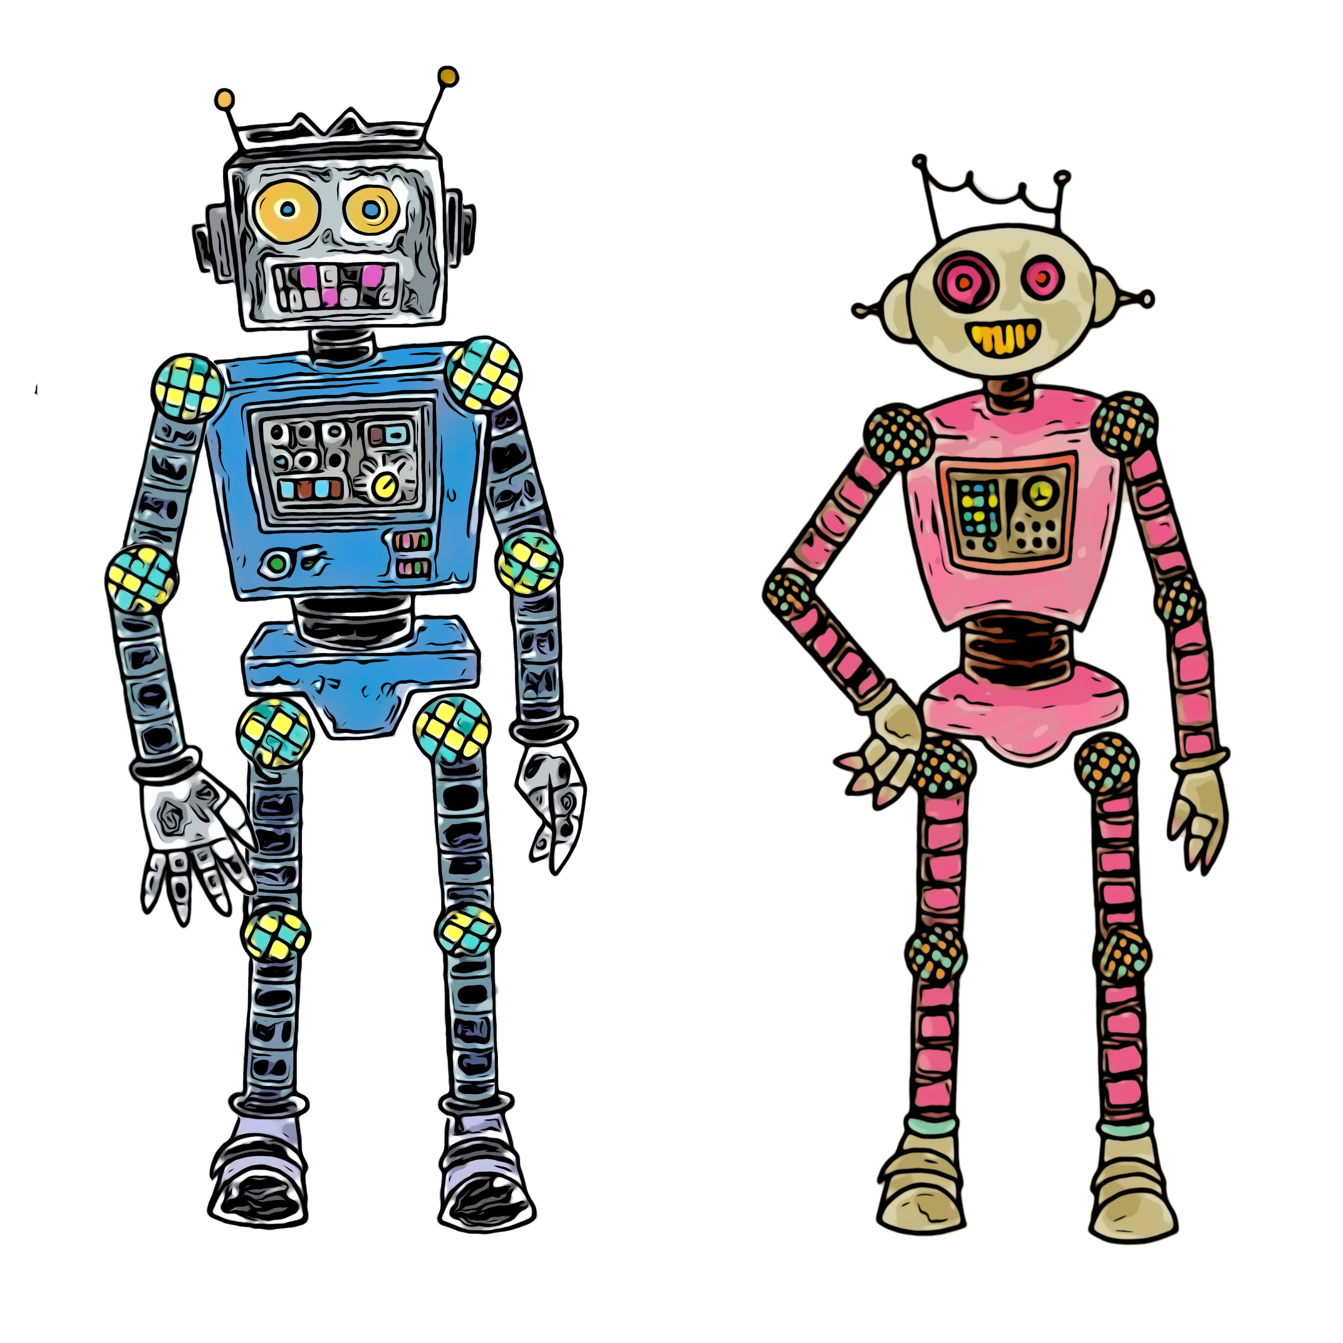
\includegraphics[keepaspectratio]{resources/images/image15.png}}

\textbf{Spielgrafik 2:} ‚Pulp`

\pandocbounded{
\includegraphics[keepaspectratio]{resources/images/image16.png}}

\textbf{Spielgrafik 3:} ‚Emmi` und ‚Sertan`

\pandocbounded{
\includegraphics[keepaspectratio]{resources/images/image17.png}}

\textbf{Spielgrafik 4:} ‚BenBox` und ‚Kleaner`

\pandocbounded{
\includegraphics[keepaspectratio]{resources/images/image18.png}}

\pandocbounded{
\includegraphics[keepaspectratio]{resources/images/image19.png}}

\textbf{Spielgrafik 5:} ‚Maschinenraum`

\pandocbounded{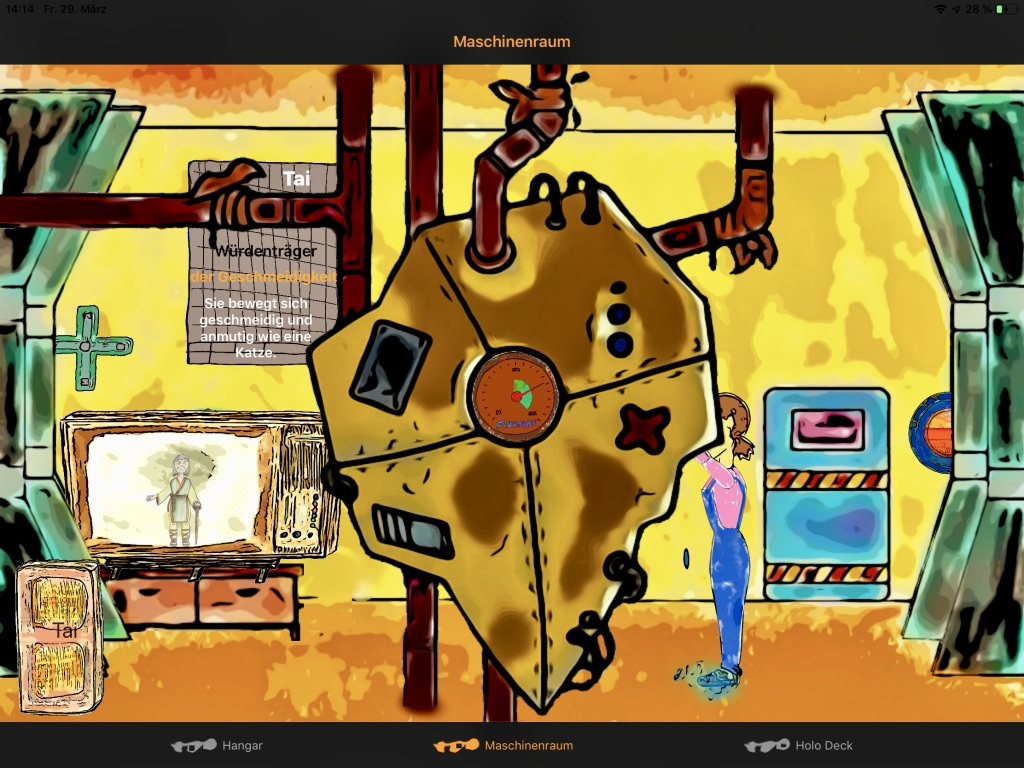
\includegraphics[keepaspectratio]{resources/images/image20.jpeg}}

\textbf{Spielgrafik 6:} ‚Hangar`

\pandocbounded{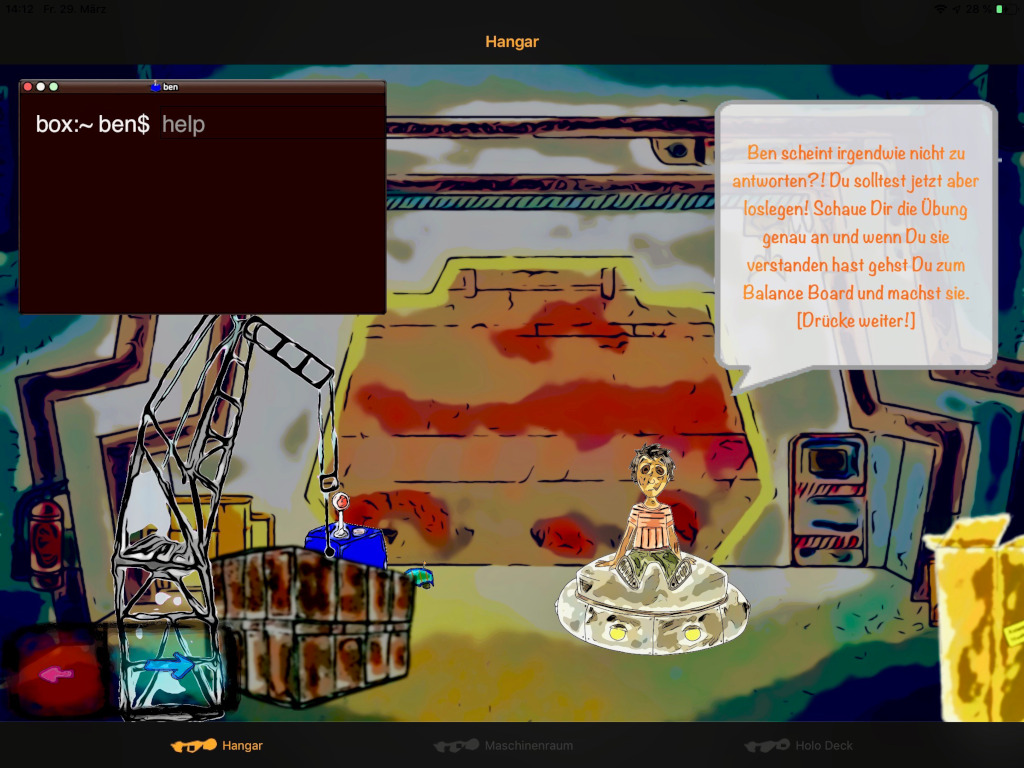
\includegraphics[keepaspectratio]{resources/images/image21.jpeg}}

\textbf{Spielgrafik 7:} ‚Holo Deck`

\pandocbounded{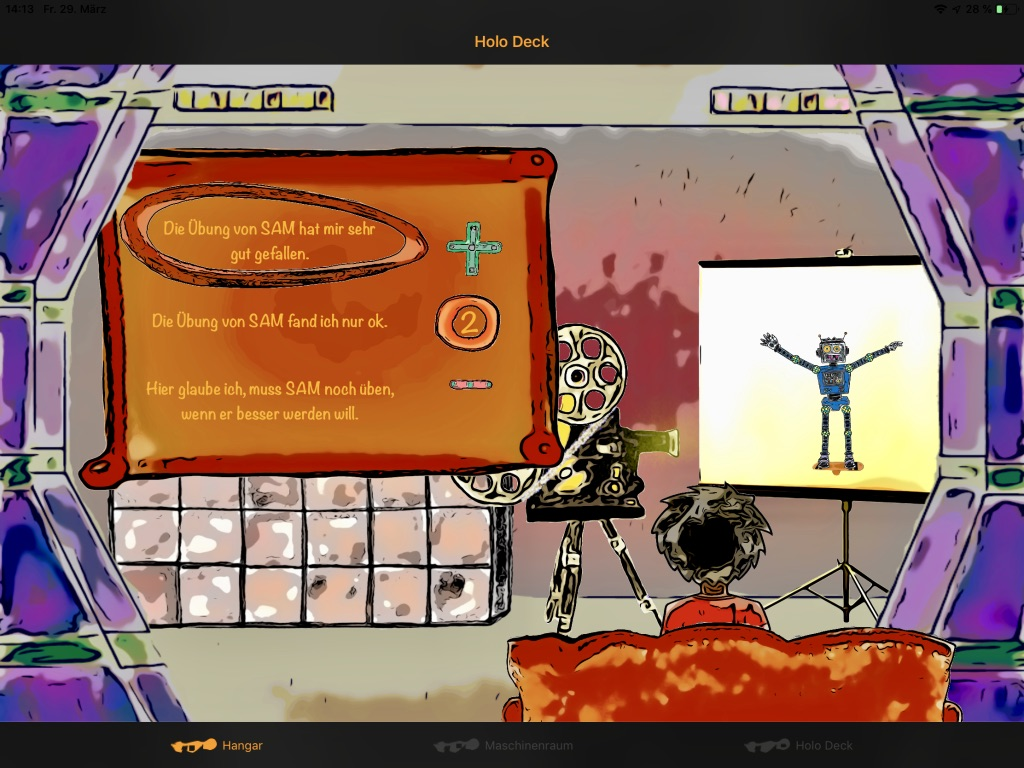
\includegraphics[keepaspectratio]{resources/images/image22.jpeg}}

\textbf{Spielgrafik 8:} ‚BenBox Protokolle`

\pandocbounded{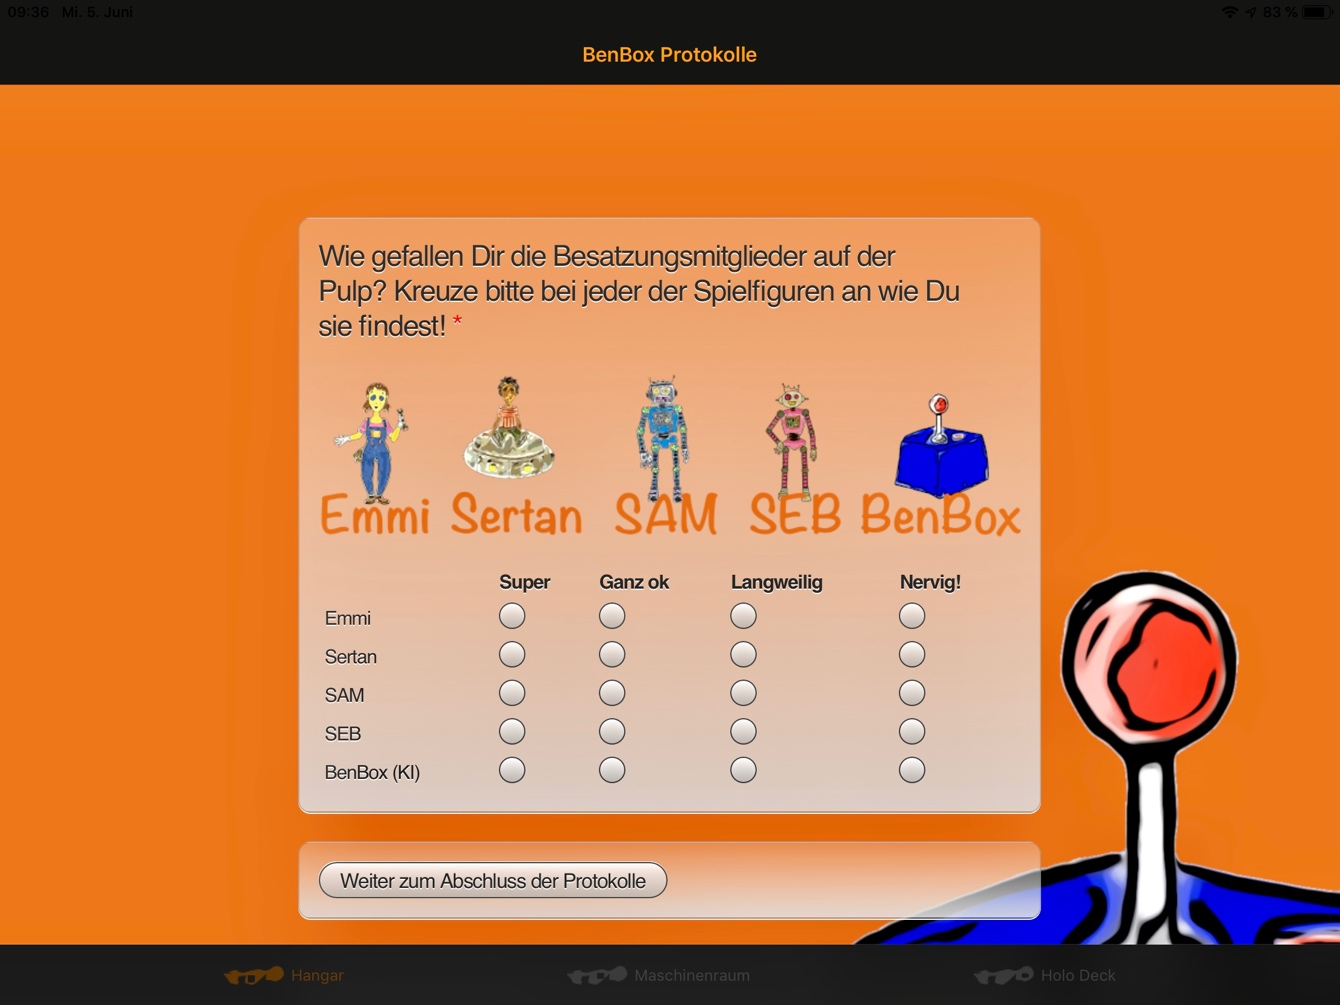
\includegraphics[keepaspectratio]{resources/images/image23.jpeg}}

\textbf{Spielgrafik 9:} ‚Via Sacra`

\pandocbounded{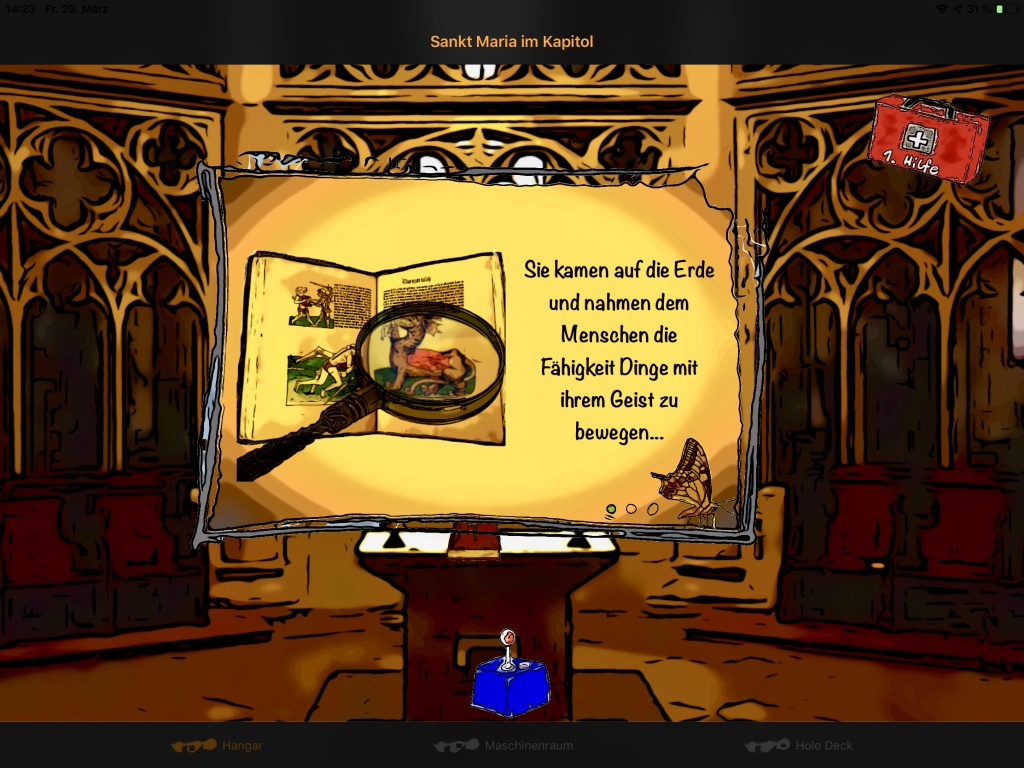
\includegraphics[keepaspectratio]{resources/images/image24.jpeg}}

\textbf{Spielgrafik 10:} ‚Updater`

\pandocbounded{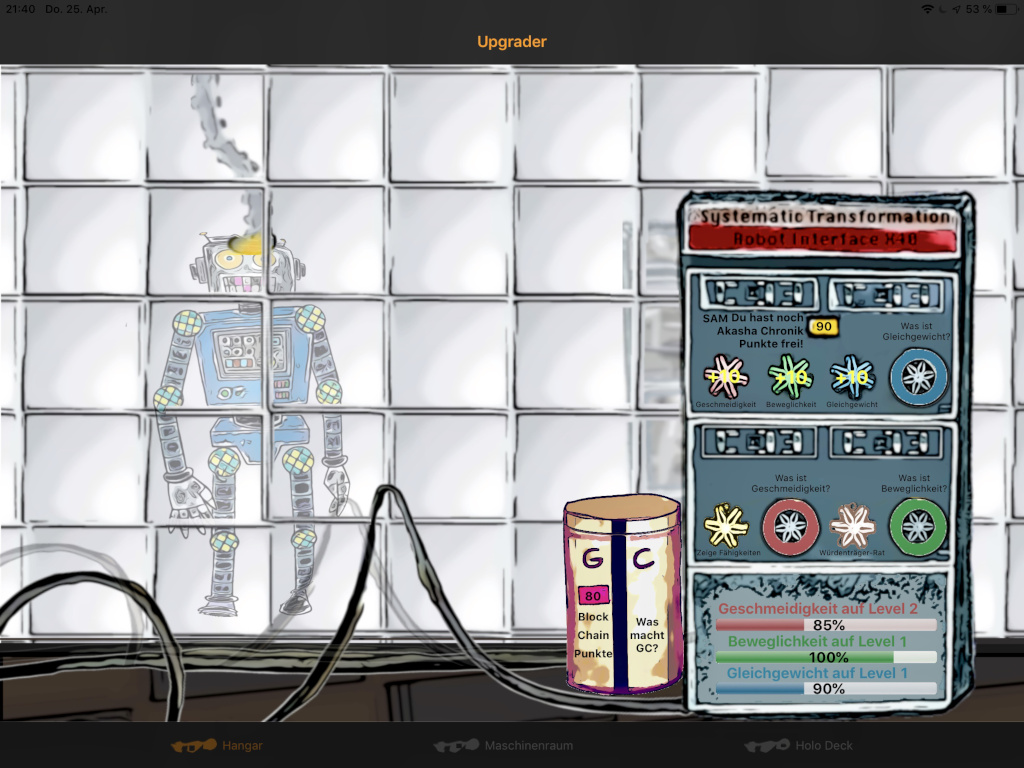
\includegraphics[keepaspectratio]{resources/images/image25.jpeg}}

\textbf{Spielkarten:} Auswahl

\pandocbounded{
\includegraphics[keepaspectratio]{resources/images/image26.png}}

\textbf{Spielgegenstände:} BenBox Balance Board und Kirchenmauer

\pandocbounded{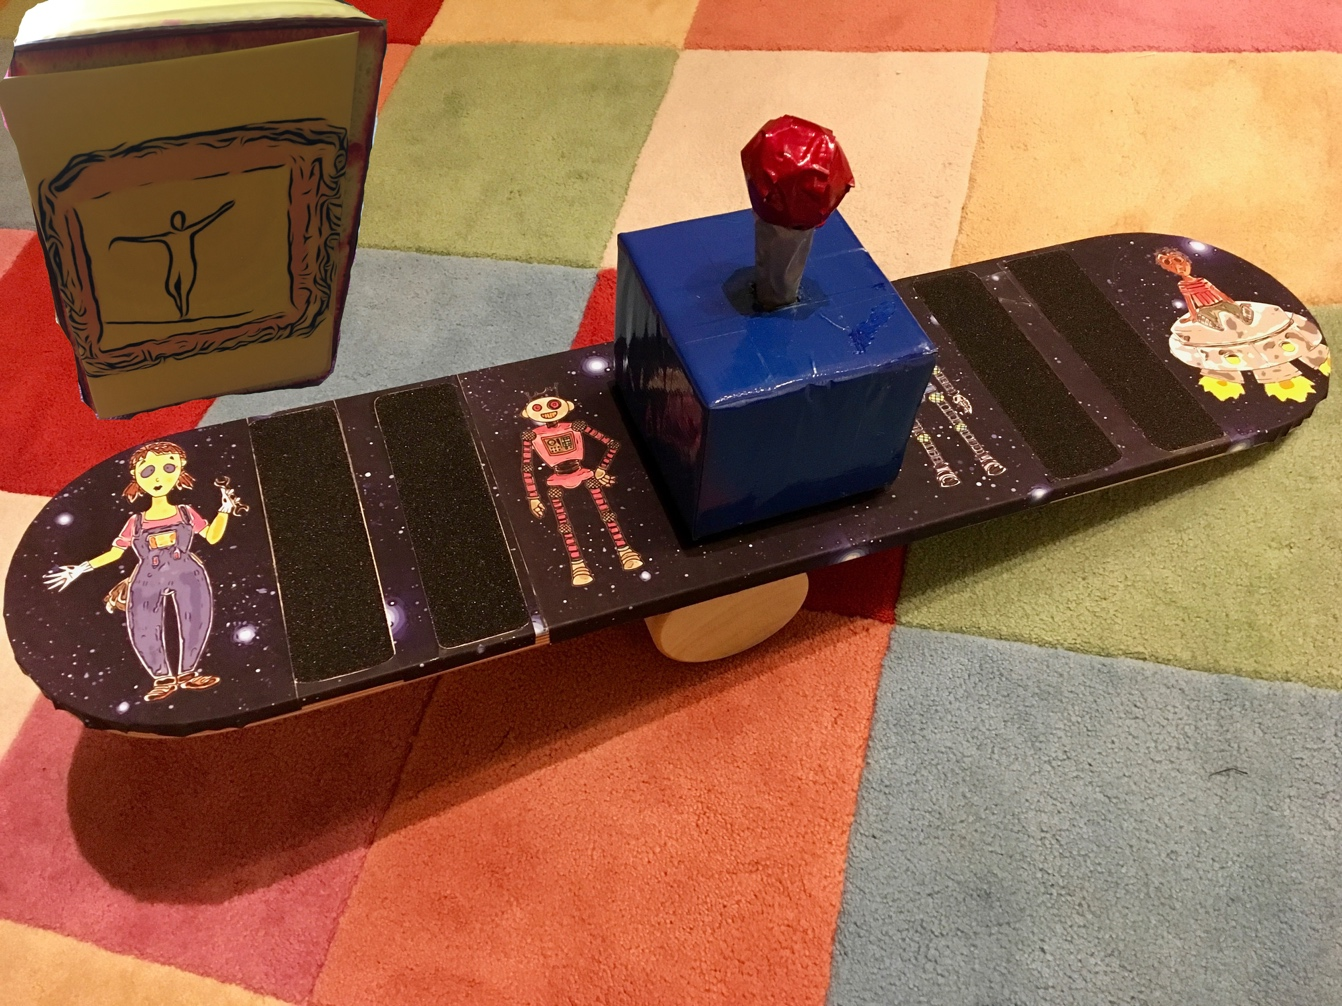
\includegraphics[keepaspectratio]{resources/images/image27.jpeg}}

\textbf{Spielgegenstände 2:} Bewertungsregeln

\pandocbounded{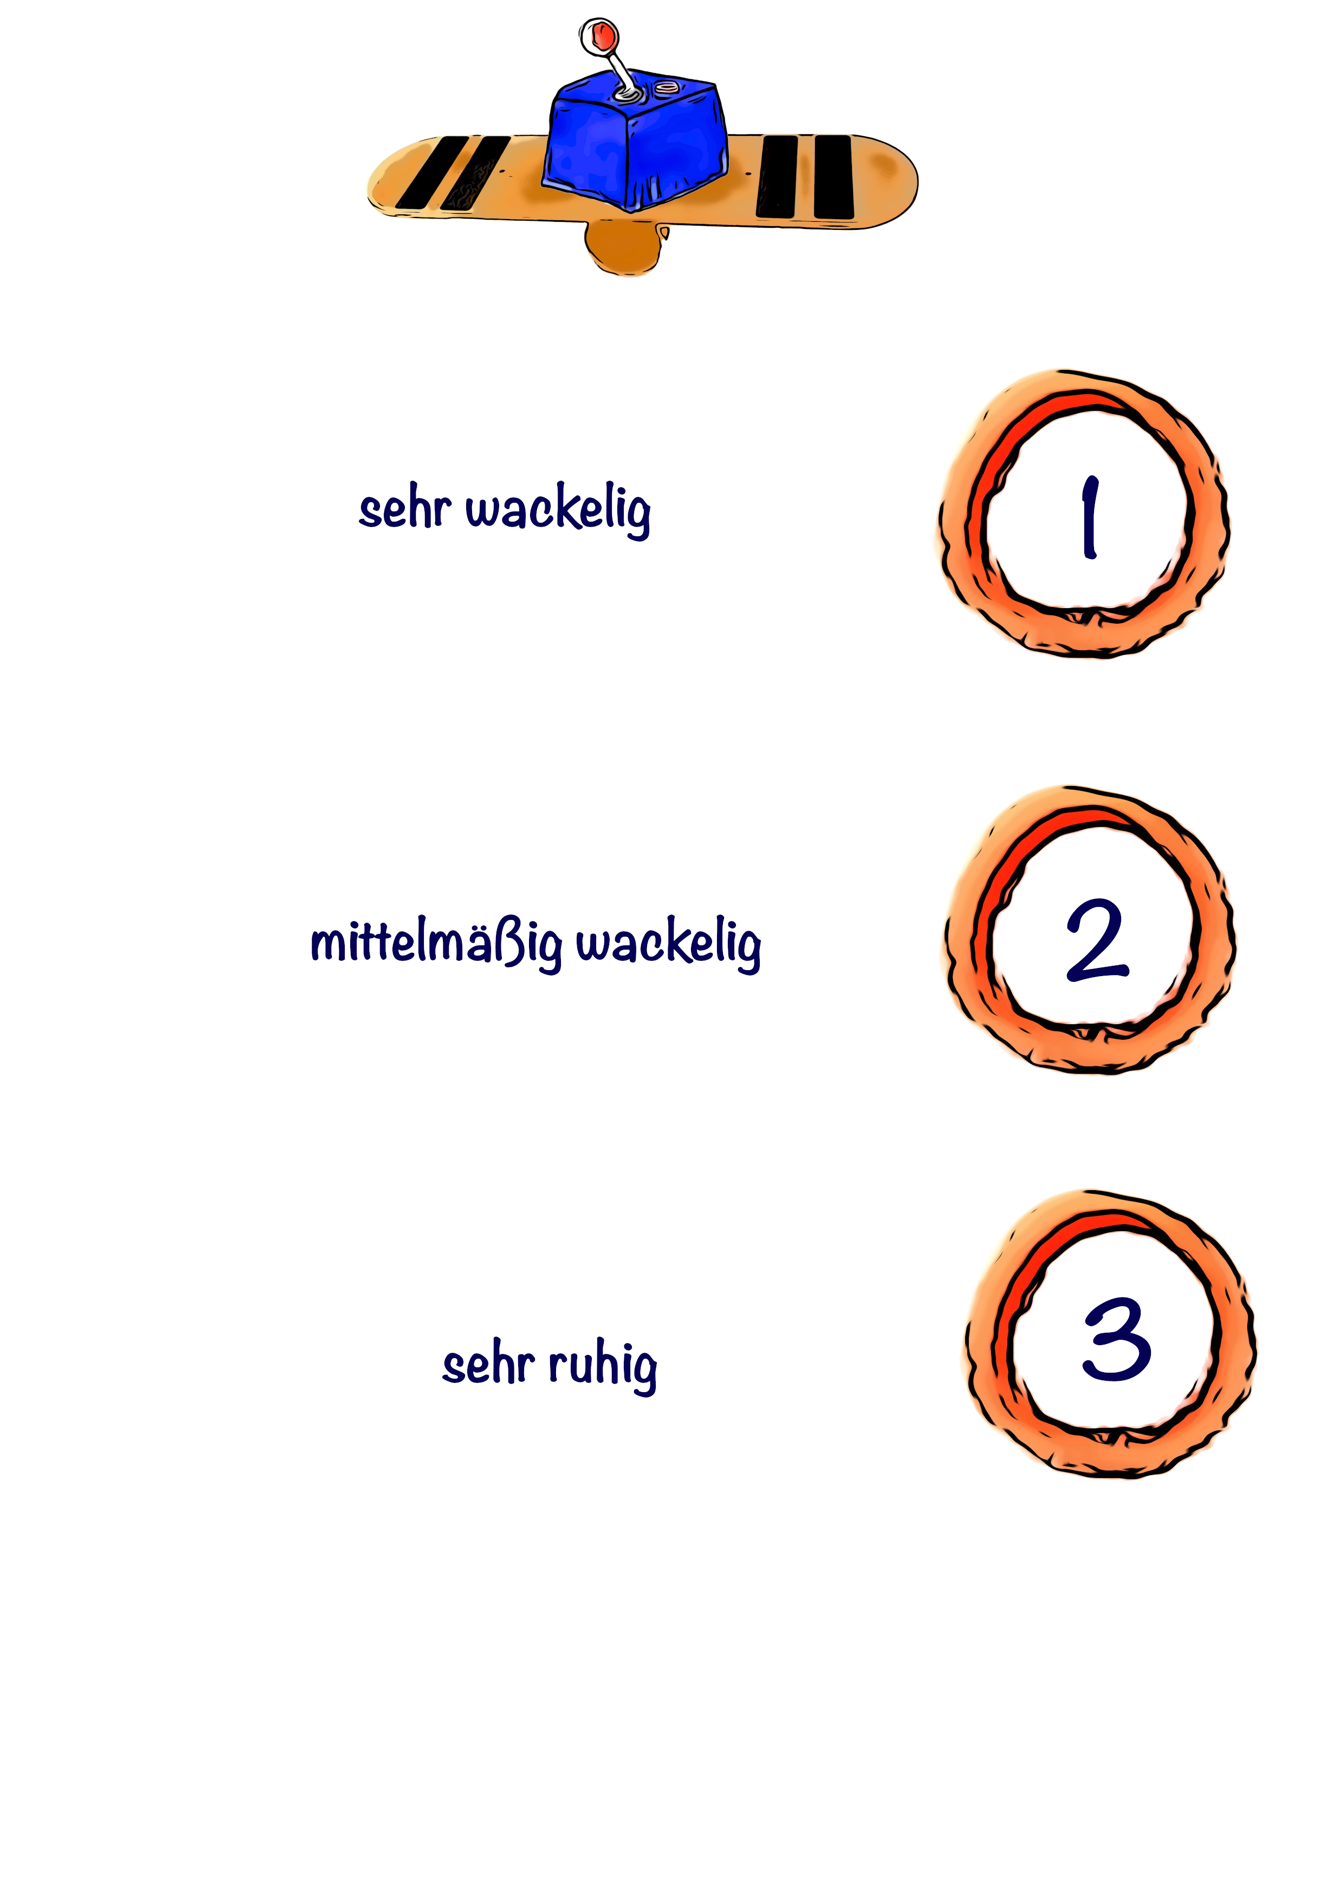
\includegraphics[keepaspectratio]{resources/images/image28.png}}

\section{Eidesstattliche
Versicherung}\label{eidesstattliche-versicherung}

Hiermit versichere ich, dass ich die vorliegende Bachelorarbeit mit dem
Titel „BenBox.org Untersuchung eines 'Serious Game` in Bezug auf seinen
Nutzen in der Gesundheitsförderung`` selbstständig und ohne fremde Hilfe
verfasst habe und keine anderen als die angegebenen Hilfsmittel
verwendet wurden.

Die Stellen der Bachelorarbeit, einschließlich der Tabellen und
Abbildungen, die anderen Werken dem Wortlaut oder dem Sinn nach
entnommen sind, habe ich in jedem Fall kenntlich gemacht und die
Herkunft nachgewiesen.

Die Bachelorarbeit hat in gleicher oder ähnlicher Form noch keiner
anderen Prüfungsbehörde vorgelegen und wurde auch noch nicht
veröffentlicht.

Köln, den Unterschrift:




\end{document}
